\documentclass[11pt]{article}

\usepackage{graphicx}
\usepackage{amsmath}
\usepackage{amssymb}
\usepackage{booktabs}
\usepackage{multirow}
\usepackage{colortbl}
\usepackage{tabularx}
\usepackage{placeins}
\usepackage{float}
\usepackage[a4paper,margin=25mm]{geometry}
\usepackage[numbers,sort&compress]{natbib}
\usepackage{setspace}
\usepackage[hidelinks]{hyperref}
\providecommand{\bibcommenthead}{}

\doublespacing
\setlength{\parindent}{1.5em}
\setlength{\parskip}{0pt}
\setcounter{secnumdepth}{0}
\pagestyle{plain}

\definecolor{TableHeader}{gray}{0.92}
\definecolor{TableAccent}{gray}{0.96}
\newcommand{\MSOTableSetup}{%
  \scriptsize
  \setlength{\tabcolsep}{2.5pt}%
  \renewcommand{\arraystretch}{1.06}%
}

% Modest float and display spacing adjustments; the journal class controls the
% page geometry, fonts, headings, and reference style.
\setlength{\textfloatsep}{8pt plus 2pt minus 2pt}
\setlength{\floatsep}{8pt plus 2pt minus 2pt}
\setlength{\intextsep}{8pt plus 2pt minus 2pt}
\setlength{\abovecaptionskip}{3pt}
\setlength{\belowcaptionskip}{0pt}
\setlength{\abovedisplayskip}{4pt plus 1pt minus 1pt}
\setlength{\belowdisplayskip}{4pt plus 1pt minus 1pt}
\setlength{\abovedisplayshortskip}{2pt plus 1pt minus 1pt}
\setlength{\belowdisplayshortskip}{2pt plus 1pt minus 1pt}
\setcounter{topnumber}{5}
\setcounter{bottomnumber}{3}
\setcounter{totalnumber}{8}
\renewcommand{\topfraction}{0.95}
\renewcommand{\bottomfraction}{0.85}
\renewcommand{\textfraction}{0.05}
\renewcommand{\floatpagefraction}{0.92}

\begin{document}
\title{Lightweight Local Map Prediction and Fusion for Resource-Constrained Multirobot Exploration}

\author{\parbox{0.95\textwidth}{\centering Haojia Gao$^{1,\dagger}$, Haohua Que$^{2,3,\dagger}$, Rongze Zhao$^{2}$,
Qian Zhang$^{2,3}$, Mingkai Liu$^{4}$, Jiajun Sun$^{2}$, Weihao Shan$^{2}$,
Hoiian Au$^{2}$, Chunhong Yuan$^{2}$, Yusen Qin$^{5}$, Rong Zhao$^{2}$,
Lei Mu$^{2}$, Bokui Chen$^{1,6}$, Xueqian Wang$^{1}$, Qi Wei$^{7}$,
Fei Qiao$^{2,*}$\\[0.75em]
\small $^{1}$Tsinghua Shenzhen International Graduate School, Tsinghua University, Shenzhen 518055, China\\
\small $^{2}$Sense Lab, Department of Electronic Engineering, Tsinghua University, Beijing 100084, China\\
\small $^{3}$Infinity Robotics, Beijing, China\\
\small $^{4}$School of Software and Microelectronics, Peking University, Beijing 102600, China\\
\small $^{5}$D-Robotics, Beijing, China\\
\small $^{6}$Peng Cheng Laboratory, Shenzhen, China\\
\small $^{7}$Engineering Research Center for Navigation Technology, Tsinghua University, Beijing 100084, China\\[0.5em]
\small $^{\dagger}$These authors contributed equally to this work.\\
\small $^{*}$Correspondence: qiaofei@tsinghua.edu.cn}}
\date{}

\maketitle

\begin{abstract}
Resource-constrained multirobot exploration can use predicted structure to reason beyond measured overlap, but predictions should not automatically authorise persistent map changes. We present Make Sense at Once (MSO), a design and retrospective audit that separates local completion, pairwise transform proposal, offline pre-commit acceptance and observation-constrained planning. A 342.8K-parameter predictor has favourable historical whole-crop point estimates relative to the evaluated backbones, although the exact split and manuscript checkpoint were not recovered. In a one-scene offline audit, probability-preserving grids yield median translation and yaw errors of 0.047\,m and 0.066$^{\circ}$, while observed occupancy yields lower median errors; the offline pre-commit acceptance gate accepts one positive outside the translation limit and rejects three positives. A separate harness rejects 150 fixed erroneous proposals before simulated map mutation. Retained aggregate simulations and one run per method in three always-connected two-robot arenas provide bounded demonstrations, not validation of the proposed gate in the deployed path. Deployed registration reliability, causal predictive benefit, building generalisation and physical scaling remain open.
\end{abstract}

%===============================================================================

\section{Introduction} \label{sec::intro}

Robots exploring an unknown environment must decide where to move before the environment has been fully observed, from search-and-rescue to planetary missions~\citep{davids2002urban,vogele2024robotics}. Classical frontier methods expand an occupancy map from measured free--unknown boundaries~\citep{yamauchi1997frontier,scherer2022resilient,umari2017autonomous}, while receding-horizon, uncertainty-aware and map-quality objectives prioritise different aspects of the same sensing problem~\citep{bircher2016receding,vallve2014dense,lehner2017exploration}. Multiple robots can reduce exploration time through parallel coverage and task allocation~\citep{matos2024efficient,long2018towards,dias2006market,yu2016optimal,gautam2012review,farinelli2004multirobot}, but doing so without a shared frame requires sensing, prediction, relative-map alignment and planning to remain mutually consistent.

Learned map completion offers a way to reason beyond the current sensor footprint~\citep{stolzle2022reconstructing,triest2024unrealnet,shrestha2019learned,georgakis2022uncertainty,ramakrishnan2020occupancy,sharma2024pre,katyal2019uncertainty,gao2025mapping}. This line of work inherits the image-inpainting problem~\citep{bertalmio2000image}: classical partial-differential-equation and patch-based methods propagate local structure or texture~\citep{bertalmio2003simultaneous,tschumperle2005vector,efros1999texture,barnes2009patchmatch}, whereas learned semantic, convolutional and transformer models capture higher-level spatial priors~\citep{song2018spg,pathak2016context,liu2018image,yan2018shift,hosen2022masked,dong2022cswin,shamsolmoali2023transinpaint}. MapEx and PIPE use global map predictions to construct probabilistic or pathwise information objectives for single-robot exploration~\citep{ho2024mapex,baek2025pipe}. Predictive multirobot work instead studies diffusion-based completion or generative-entropy coordination~\citep{tan20244cnet,spinos2025map}. These studies focus on prediction and target allocation rather than accepting a pairwise map transform under an initially unknown interrobot frame. Global completion and generative models~\citep{goodfellow2014generative} can also be expensive for embedded hardware~\citep{kamath2023deep,goyal2004lightweight,que2026motimem}. More importantly, predicted walls are hypotheses rather than measurements: they may provide alignment cues, but hallucinated or repeated structure can produce a plausible wrong match.

Multirobot exploration has consequently combined distributed information objectives~\citep{mu2016information,wang2025multi} with frontier search~\citep{holz2010evaluating,dornhege2013frontier}, rapidly exploring trees and graphs~\citep{lavalle1998rapidly,karaman2011sampling}, hybrid sampling policies~\citep{selin2019efficient,respall2021fast}, topological coverage~\citep{choset2000sensor,acar2002sensor} and information-theoretic planning~\citep{bourgault2002information,stachniss2005information}. In practical rendezvous, a robot's mapped region can remain smaller than its communication range, so first contact need not provide sufficient observed overlap for direct registration~\citep{zhou2006multi,thrun2005multi,birk2006merging,stathoulopoulos2023frame}.

Collaborative localisation and mapping systems address interrobot constraints through loop closure, robust estimation and pose-graph optimisation~\citep{lajoie2020door,schmuck2019ccm,lajoie2024swarm}; Swarm-SLAM, for example, provides a sparse decentralised collaborative-SLAM framework rather than a learned occupancy-completion or exploration policy~\citep{lajoie2024swarm}. Direct observation of peer robots provides another source of relative pose but depends on visibility~\citep{wang2024transformloc,zhu2024swarm,zhou2022swarm}. Occupancy-map registration offers a pairwise route when robots do not initially share a frame, using particle-filter, expectation-maximisation, clustering or learned matching formulations~\citep{carlone2011simultaneous,huang2024multi,dong2015distributed,saeedi2011multiple,saeedi2011neural}. The question addressed here is narrower: how can a small local predictor interact with transform proposal, offline pre-commit acceptance and persistent-map authority on resource-constrained robots?

A recent visual cooperative-SLAM study with one overlapping author addresses trajectory relocalisation under tracking loss and communication constraints. It uses historical keyframes, locally optimised frame dropping and a communication buffer, evaluated with TUM Mono-VO sequence replays against CCM-SLAM~\citep{chen2026accurate}. MSO instead studies provisional two-dimensional occupancy completion, pairwise map-transform proposal and observation-constrained exploration using KTH/HouseExpo records, a mobile-robot local-planning benchmark simulation and LiDAR arena logs. The public MSO dependency record does not identify the visual-SLAM implementation as a software dependency. We therefore distinguish the studies by scientific question, declared software dependency, evaluation data, reported experiments and claim: MSO makes no visual-SLAM back-end or communication-buffer contribution.

Here we ask how compact prediction, pairwise alignment, offline pre-commit acceptance and observation-constrained planning can be organised without granting predictions authority over persistent state. We present \emph{Make Sense at Once (MSO)}, a two-dimensional indoor architecture that co-designs these four functions (Fig.~\ref{fig1}). Building on our earlier single-robot local-prediction work~\citep{gao2025senseexpo,gao2025mapping}, MSO specifies a 342.8K-parameter distilled predictor and an ambiguity-heuristic, multi-scale transform proposal. A temporary leader and pose graph are implementation mechanisms rather than contributions.

The contribution is an auditable architecture and evidence map for linking learned completion to relative-map alignment and observation-constrained multirobot exploration while preserving measurement authority. Specifically:
\begin{itemize}
	\item We specify resource, geometry and mapping-authority contracts across a compact local predictor, pairwise transform proposal, offline pre-commit acceptance and observation-constrained planning.
	\item We audit non-equivalent preserved artefacts separately: historical predictor summaries, a reconstructed one-scene registrar, a simulated rejection-before-mutation harness and a negative replay of the legacy deployment path.
	\item We report aggregate simulations and descriptive two-robot arena runs as bounded demonstrations, with coverage, occupied-cell precision and integration limits stated explicitly.
\end{itemize}

The claim is deliberately narrower than a new generic predictor, registration algorithm or collaborative-SLAM back end. MSO focuses on the design interface among local completion, pairwise alignment under an unknown initial transform, offline pre-commit acceptance and observation-constrained planning. The current evidence does not validate those functions as one frozen deployed implementation. The direct transform audit uses a reconstructed offline reference registrar, the mutation test uses a separate harness, and the physical study records a legacy path without the proposed gate.

%===============================================================================

\section{Results} \label{sec::results}

\subsection{System design and evaluation scope} \label{sec::preliminaries}

\begin{figure}[htbp]
	\centering
	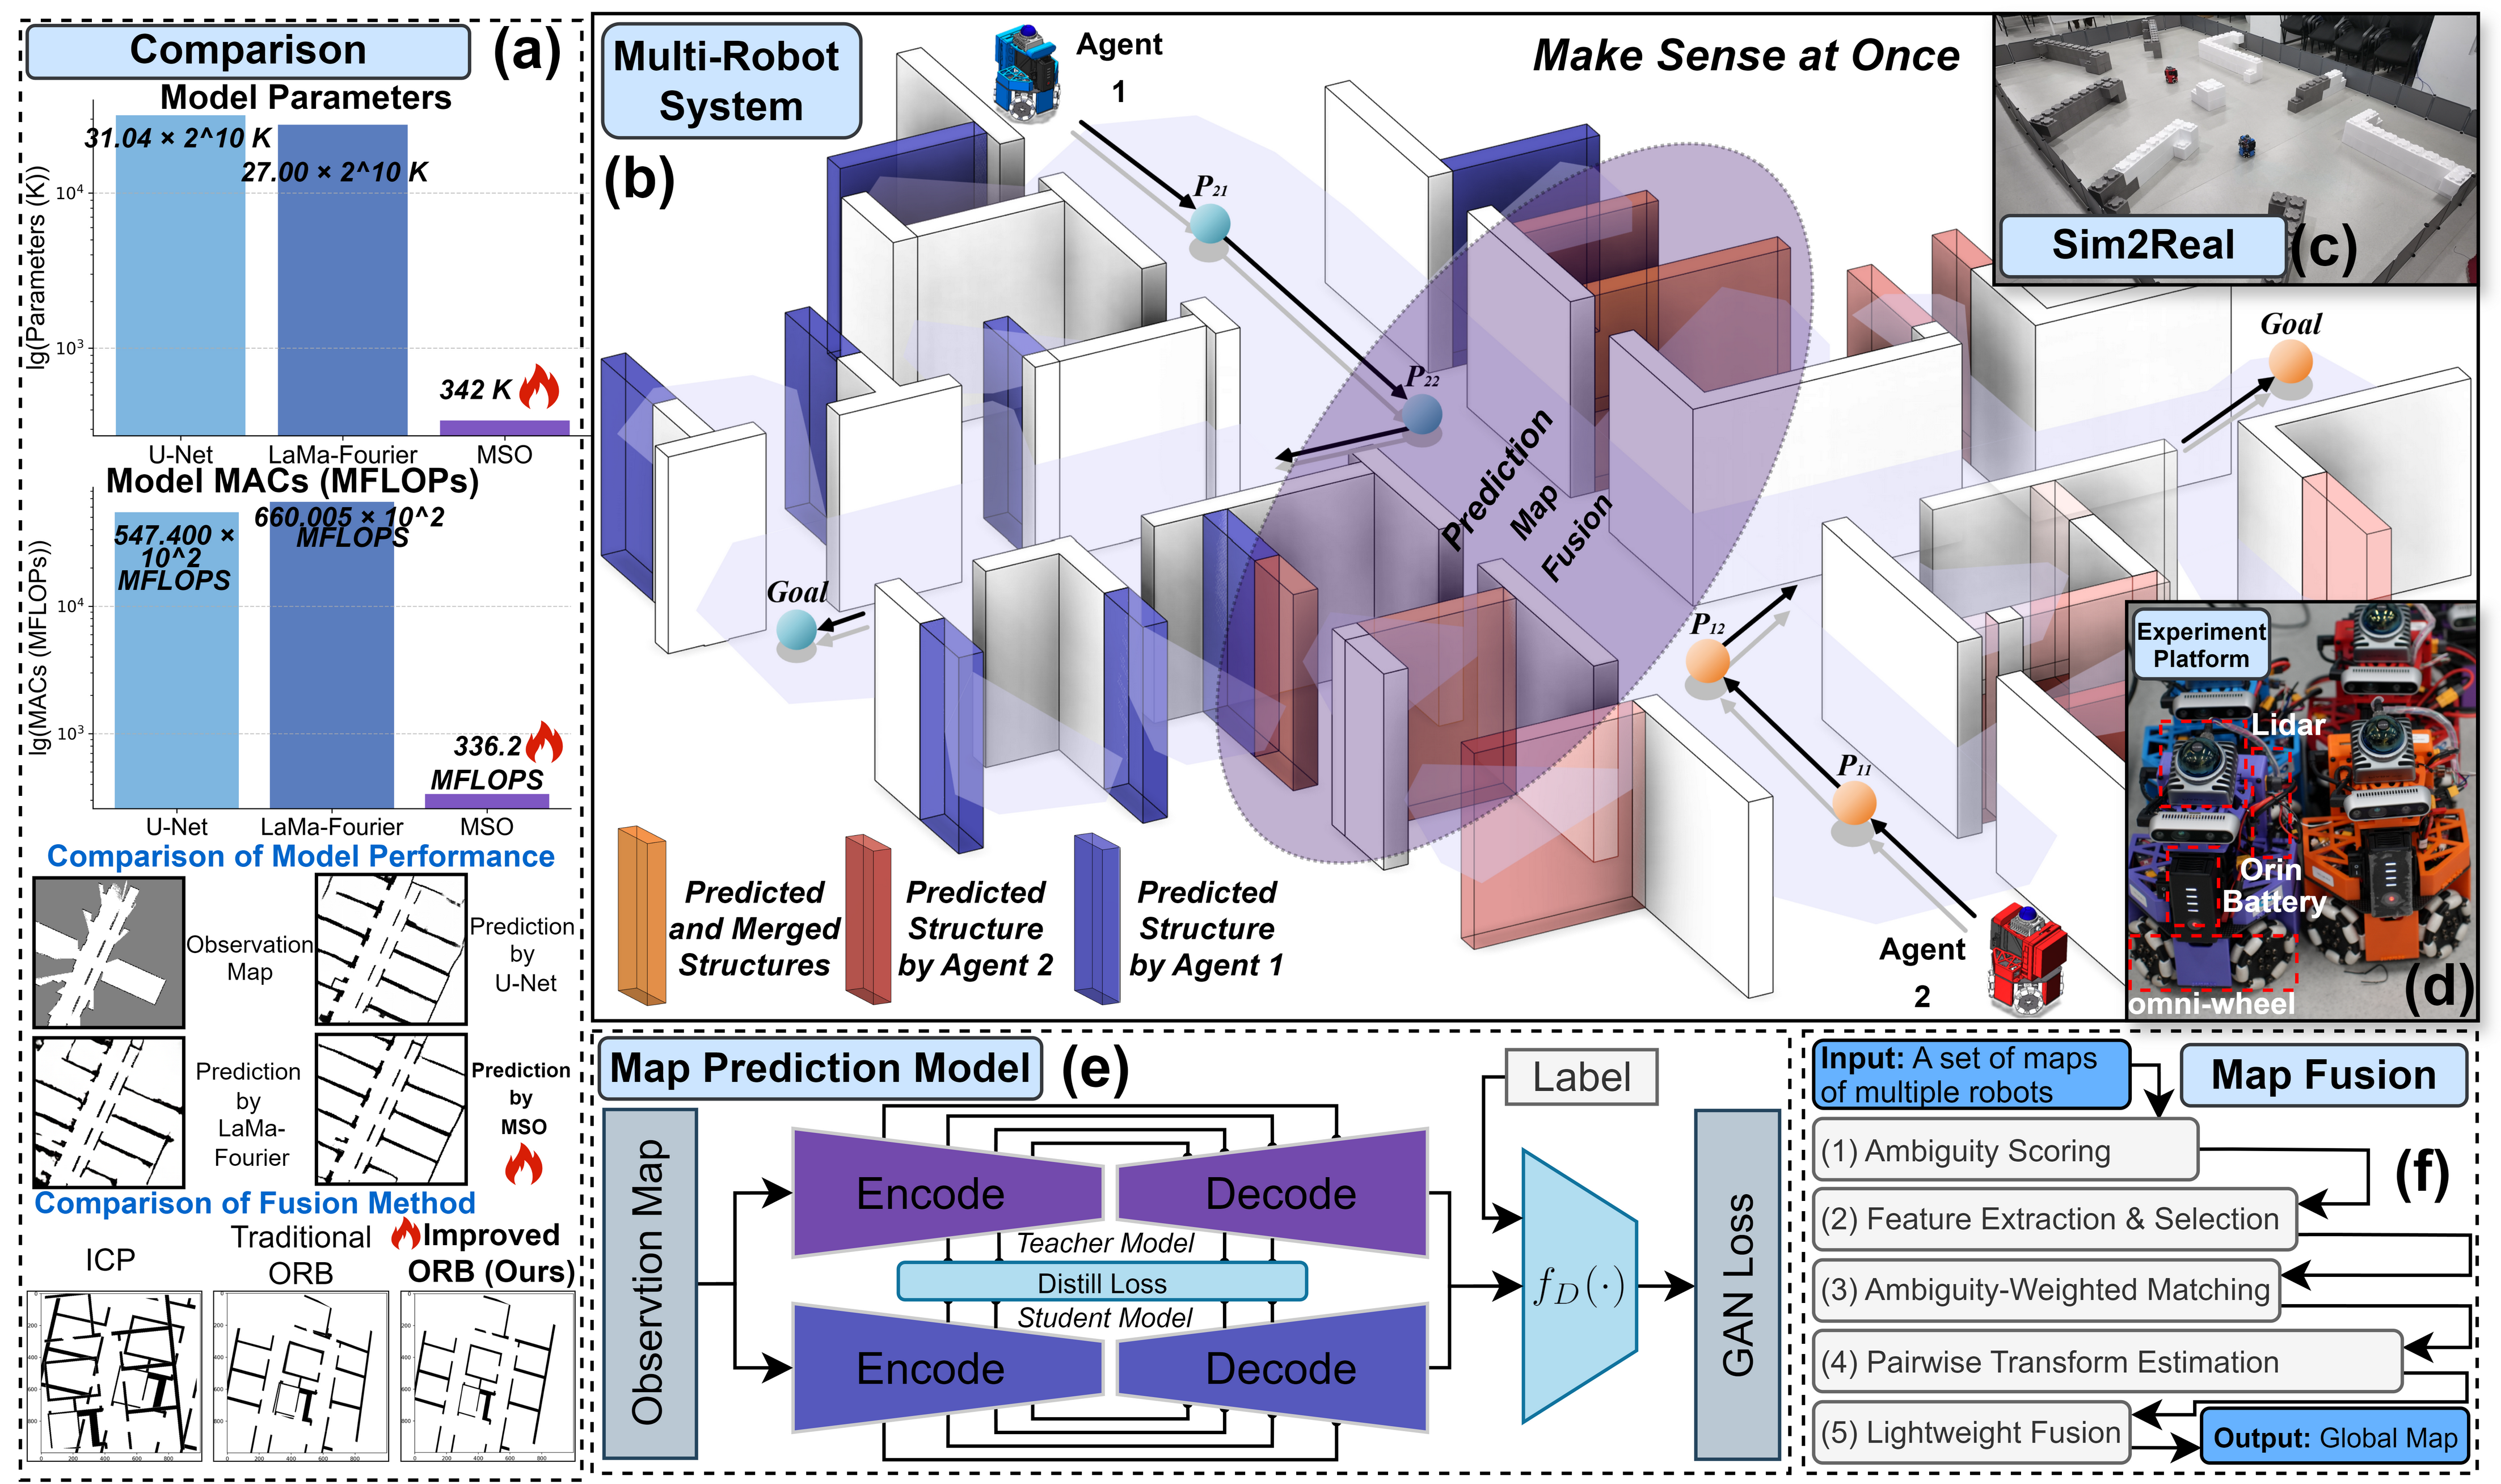
\includegraphics[width=\textwidth]{figure1.png}
	\caption{
		\textbf{MSO design and evidence overview.} \emph{a}, Reported model-size and completion-metric comparison. The original schematic's profiler wording is retained; because its counting convention was not recovered, Fig.~\ref{fig:resource-profile} and the text use the neutral term ``operation entries''. \emph{b}, Multirobot exploration with local prediction and pairwise map registration. \emph{c}, Controlled physical arena. \emph{d}, Robot platforms. \emph{e}, Teacher--student predictor. \emph{f}, Predictive-map registration pipeline. Panels depict the proposed architecture and preserved evaluation settings, not one validated deployed implementation.
	}
	\label{fig1}
\end{figure}

Figure~\ref{fig1} links four functions in the proposed architecture: local occupancy completion, pairwise transform proposal, an observed-support offline pre-commit acceptance check and exploration. Prediction can supply candidate structure for matching and target ranking, but measured occupancy remains authoritative for collision checking and persistent-map updates. The robots do not begin with a known interrobot transform. These interfaces are assessed through separate preserved artefacts rather than one validated deployed implementation. Detailed map, agent and coordinate definitions are given in Methods and Supplementary Table~1.

The evidence is organised around explicit boundaries. Completion quality comes from a historically reported crop split whose exact manifest and manuscript checkpoint are unavailable. Transform correctness is tested offline under saved two-dimensional perturbations, and rejection before mutation is tested in a separate harness. Only aggregate traces remain from simulations configured with repeated seeds. Physical operation is shown in three small, always-connected two-robot arenas using the legacy deployment path. These records support retrospective design auditing and bounded feasibility demonstrations, not end-to-end validation of the proposed gate or generalisation across buildings, unreliable networks or large robot teams.
\subsection{Evaluation data} \label{sec::datasets}
We follow Gao et al.~\citep{gao2025senseexpo,gao2025mapping}, generating samples from the HouseExpo simulator~\citep{li2020houseexpo} and KTH dataset~\citep{aydemir2012can}: a random region is sampled, two robots are spawned at random positions, and at each step the local observation is accepted if the inter-trajectory distance $dis\in[\sigma_1,\sigma_2]$ and the obstacle/free ratios fall within $[\Phi_1,\Phi_2]$ and $[\Phi_3,\Phi_4]$. Accepted samples are stored as three-channel \{\emph{Obstacles}, \emph{Uncertain}, \emph{Free}\} grids. The historical experiment record states that fitting and held-out crops did not share a parent floorplan, but the exact sample-level manifest was not recovered. The closest preserved archive contains 6{,}841 train-labelled and 1{,}463 test-labelled samples, which do not reproduce the reported 5{,}385/1{,}356 counts. These labels and the available identifiers do not support an independent parent-floorplan or building audit. The reported results are therefore descriptive historical point estimates rather than a verified floorplan-disjoint, building-disjoint or locked test-set claim. Thresholds, class statistics and this limitation are detailed under Dataset construction in Methods.

\subsection{Resource-constrained local map prediction} \label{sec::map prediction model}

\begin{figure}[htbp]
	\centering
	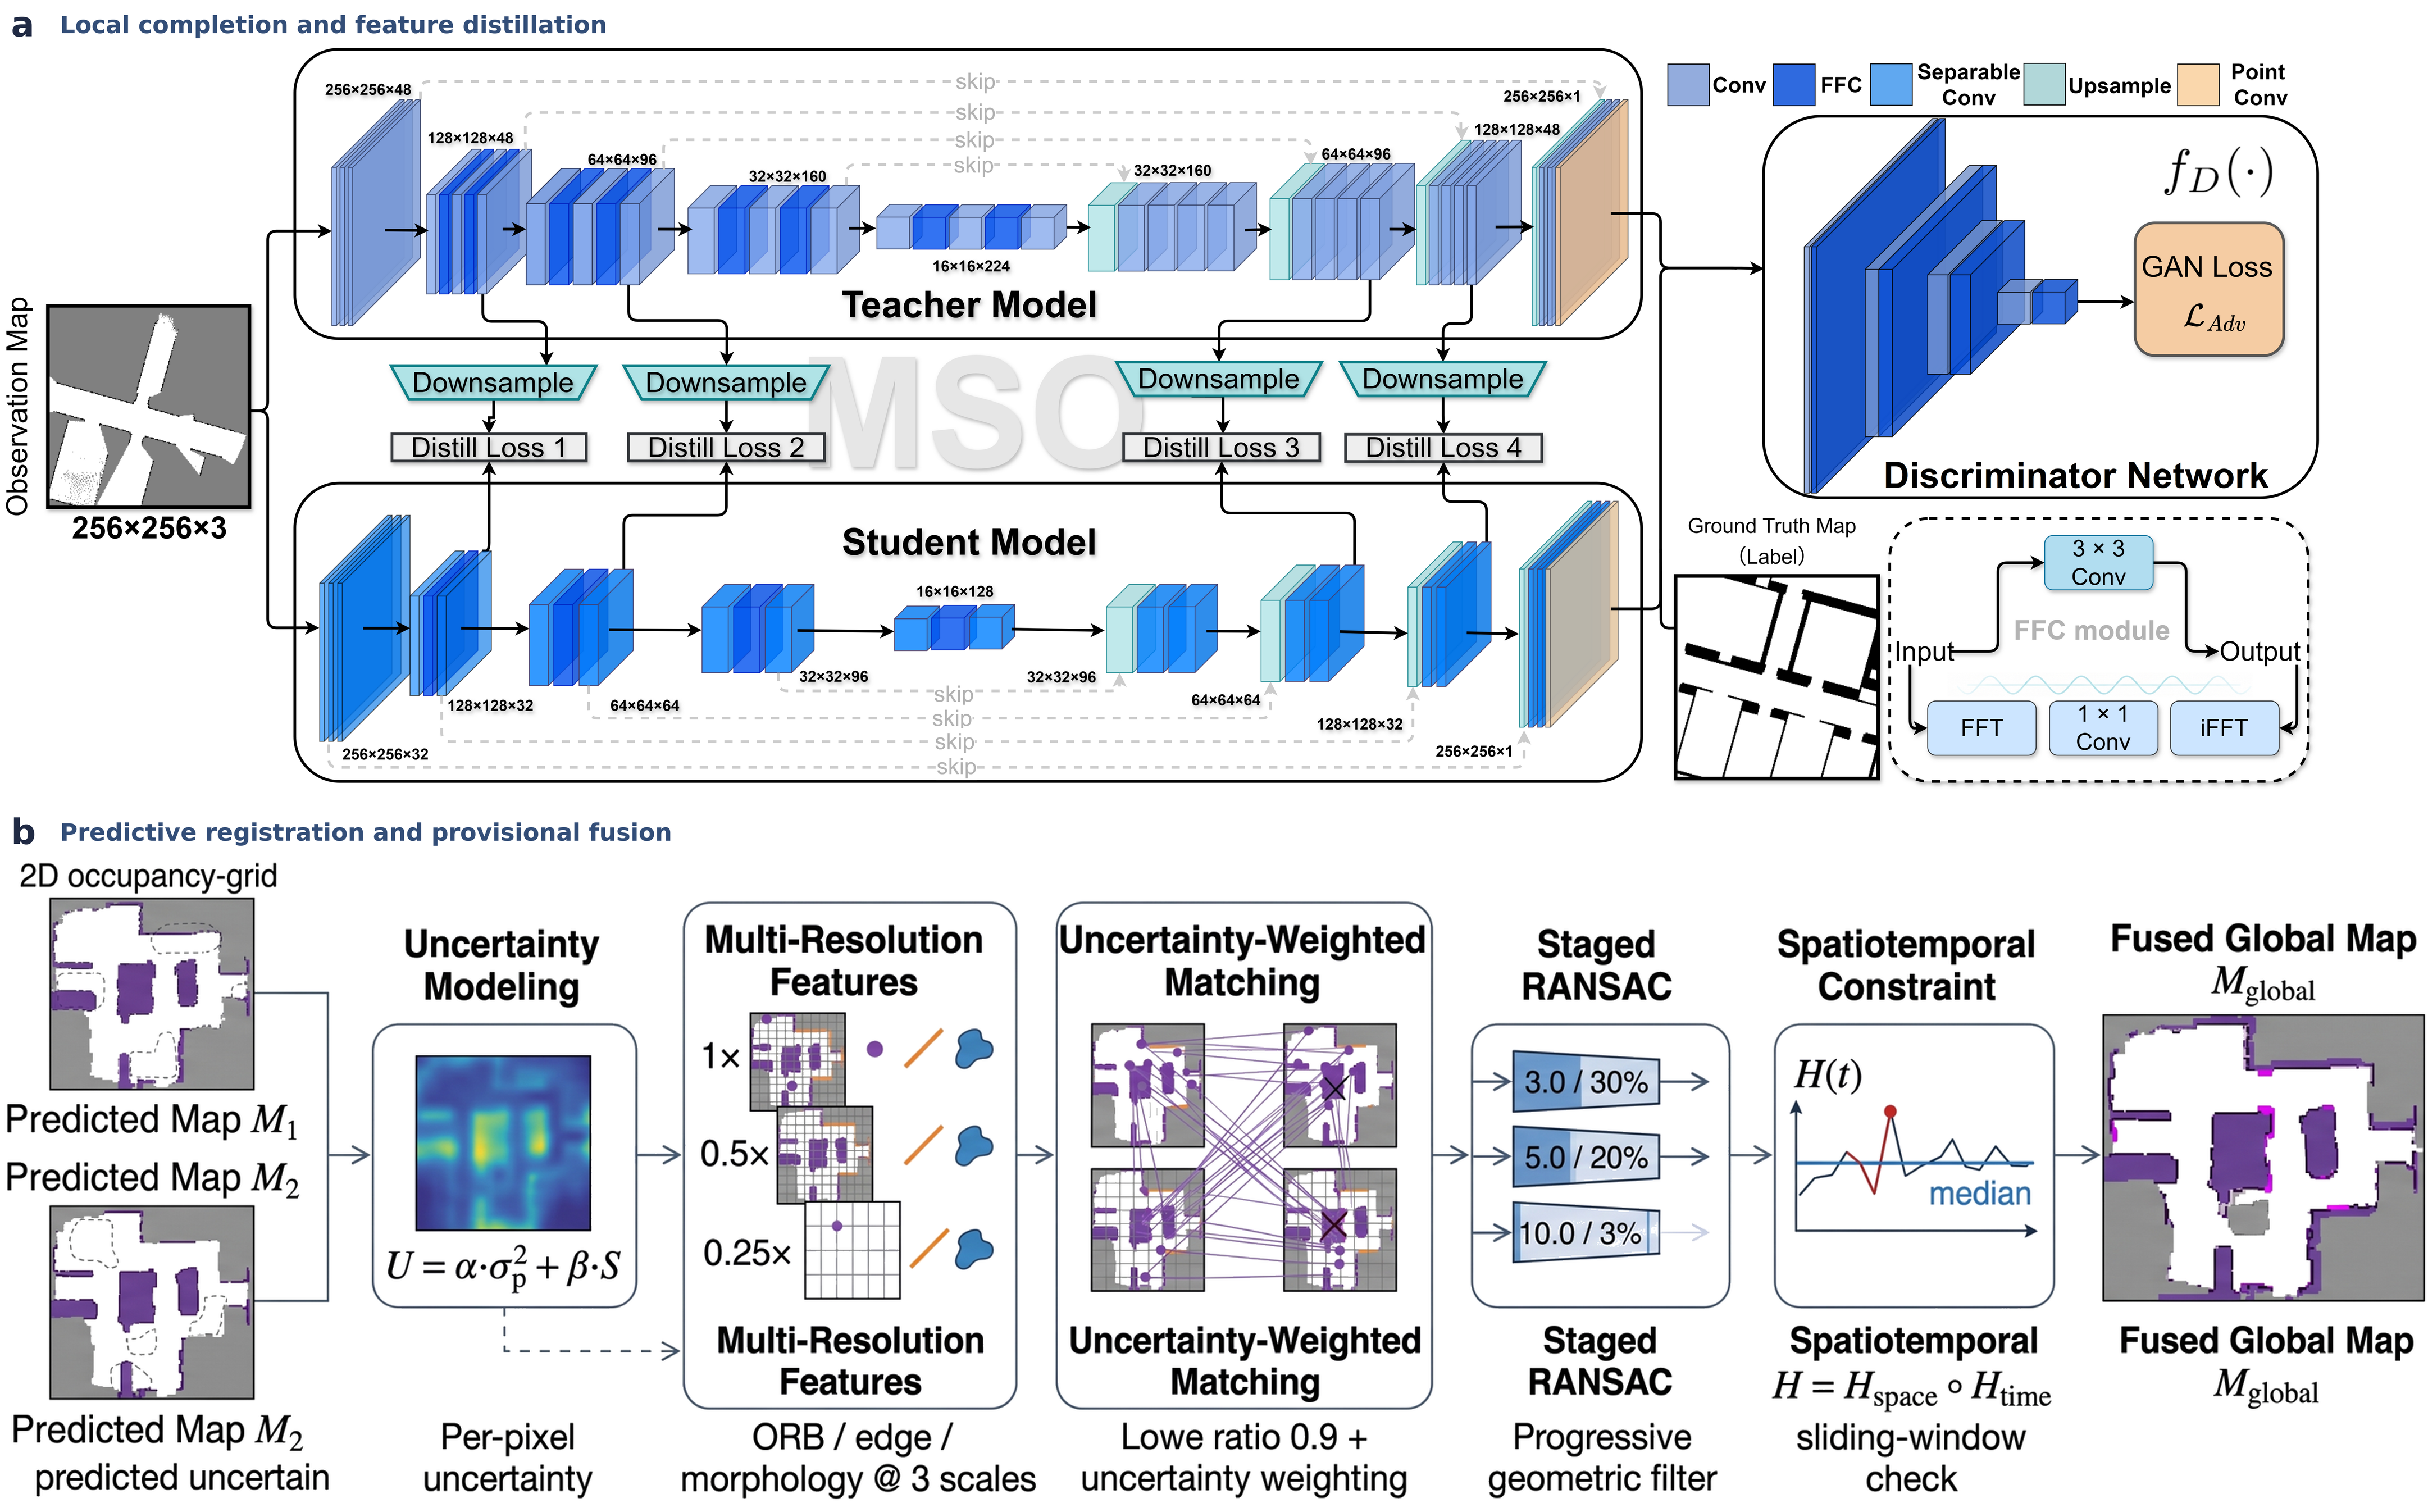
\includegraphics[width=\textwidth]{figure2_composite.png}
	\caption{\textbf{Local prediction and predictive registration workflow.} \emph{a}, A generative teacher completes the unknown part of a three-channel occupancy crop. Intermediate teacher features supervise the compact student through channel projections, while measured free and occupied cells are copied unchanged into the completed map. \emph{b}, Two provisional predicted maps are assigned a deterministic ambiguity score, decomposed into multiresolution features, matched with ambiguity weighting and filtered geometrically before a provisional transform and overlap-aware fusion are produced. Panel b is an explanatory workflow rather than experimental output.}
	\label{fig2}
\end{figure}

The predictor uses convolutional downsampling, fast Fourier convolution (FFC) modules for global context~\citep{suvorov2021resolution,chi2020fast}, and skip connections that preserve local structure~\citep{ronneberger2015u} (Fig.~\ref{fig2}).

The teacher uses additional convolutional and FFC blocks. Four projected intermediate features supervise the compact student. Both objectives combine masked adversarial, feature-matching and $L_2$ terms~\citep{suvorov2021resolution,chi2020fast,he2016deep,isola2017image,mescheder2018training}; the student also receives a feature-distillation loss. Equations and weights are reported under Training objectives in Methods.


\subsection{Predictive map registration and acceptance boundary} \label{sec::map fusion}
Predictive map fusion differs from classical occupancy-grid stitching because the inputs contain both observed structure and model-generated hypotheses. We therefore evaluate two components: an ambiguity heuristic for predicted regions and multi-resolution computation suitable for onboard use. The per-pair matcher (Fig.~\ref{fig1}(f); Supplementary Algorithm~1) combines this heuristic with staged geometric verification and multi-resolution alignment.

\paragraph{Ambiguity heuristic and feature selection.}
At each pixel the deterministic student outputs one occupied-cell probability $\hat p(x,y)$. We use the pixelwise Bernoulli variance $\sigma_{p}^{2}=\hat p(1-\hat p)$ as a single-pass ambiguity heuristic; it is not a calibrated estimate of epistemic uncertainty. Observed cells are assigned a zero heuristic value. The feature-rejection score is $\mathcal{U}(x,y)=\alpha\sigma_{p}^{2}(x,y)+\beta\mathcal{S}(x,y)$ with $\alpha{=}0.7$, $\beta{=}0.3$, where $\mathcal{S}$ is a binary normalised Canny response used as an additional boundary-instability penalty. Consequently, lower scores are retained; this sign convention is deterministic rather than probabilistic. We extract oriented FAST and rotated BRIEF (ORB), edge and morphological features at three scales ($1\times,0.5\times,0.25\times$) and keep features whose score falls below $0.8\,\mathrm{mean}(\mathcal{U})$. Multi-hypothesis, ensemble and pathwise uncertainty estimates are not compared.

\paragraph{Ambiguity-heuristic weighting and staged RANSAC.}
Candidate matches are scored by an ambiguity-heuristic exponential
$w_m=\exp\!\bigl(-(\mathcal{U}(k_1)+\mathcal{U}(k_2))/(2\sigma_{\mathcal{U}}^{2})\bigr)$,
where $\sigma_{\mathcal U}^{2}$ is the variance of endpoint scores over candidate matches in the current pair. The implementation uses an explicit numerical branch: if $\sigma_{\mathcal U}^{2}\leq10^{-12}$, all candidate weights are set to one; otherwise the expression above is evaluated. This is a fallback, not the mathematical zero-variance limit of the exponential. We use a Lowe ratio of $0.9$ and direct matching when fewer than eight KNN matches remain. Displacement, scale and angle filters precede staged RANSAC~\citep{fischler1981random} at $3.0/30\%$, $5.0/20\%$ and $10.0/3\%$ thresholds (5000 iterations). Full-resolution refinement is restricted to the estimated overlap. Parameters and pseudocode appear under Map fusion pipeline in Methods.

\paragraph{Scope of evaluation.}
The original pairwise benchmark evaluates registered overlap through Dice, an archived unitless RMSE summary, SSIM and a thresholded success rate. The controlled stress test in Fig.~\ref{fig:transform-audit} evaluates pose error and offline pre-commit acceptance decisions under known perturbations. It is scene-limited and based on an archived reference implementation; neither protocol establishes temporal drift, deployed commit behaviour or post-commit recovery. A separate component ablation tests the predicted-map split.

\subsection{Observation-constrained multirobot exploration design} \label{sec::multirobot-exploration}
The architecture assigns prediction and pairwise fusion to each onboard computer. Robots start at random poses, maintain observed map $M_i$ and predicted map $\hat{M}_i$, and exchange odometry, predicted maps and features in communication range (Supplementary Table~3). Each frontier cluster $c$ receives
\[
\mathrm{score}(c)=\mathrm{IG}(c)-\lambda_{d}d(c)-\lambda_{u}\mathcal{U}(c),
\]
with $(\lambda_{d},\lambda_{u})=(1.0,0.5)$. Here $\mathrm{IG}(c)$ and $\mathcal{U}(c)$ are computed in the predicted candidate view cone, whereas $d(c)$ is the A$^\star$ path length on measured map $M_i$. Thus prediction ranks targets, but path construction and collision checking use measured occupancy.

%===============================================================================

The evaluation addresses five bounded questions: historical prediction quality and cost relative to the evaluated inpainting baselines; overlap metrics for the proposed matcher relative to the tested ORB and iterative closest point (ICP) configurations; controlled relative-pose recovery and abstention in one archived scene; retained aggregate exploration coverage in one simulation layout; and legacy-path operation in controlled, always-connected two-robot arenas. The experiments do not establish cross-building or deployed online registration reliability, building-disjoint prediction generalisation, communication-failure robustness, or physical scaling beyond two robots.

\subsection{Compact local map completion} \label{sec:local-map-prediction}

\paragraph{Setting and baselines.}
The historical experiment record reports fitting on 5{,}385 and evaluating on 1{,}356 held-out local crops ($256\times256$) with Adam (lr~$=10^{-3}$, 500 epochs). Baselines are U-Net~\citep{ronneberger2015u}, LaMa-Fourier~\citep{suvorov2021resolution} and distilled MI-GAN~\citep{sargsyan2023mi}. PSNR, SSIM and LPIPS~\citep{zhang2018perceptual} are computed per complete output after observed free and occupied cells have been copied unchanged from the input; FID~\citep{heusel2017gans,obukhov2020torchfidelity} and KID~\citep{obukhov2020torchfidelity,binkowski2018demystifying} are computed over the same set of complete outputs. Observed cells account for 51.1\% of pixels on average and are identical by construction. Uncertain-region-only metrics were not retained, so these whole-crop image scores may partly reflect copied observations and do not directly measure topology, obstacle recall or navigation safety. The selected models are component baselines, not a comprehensive predictive-exploration comparison. Methods gives the reported configuration and the unresolved provenance boundary.


\paragraph{Results.} Figure~\ref{fig:resource-profile} and Supplementary Table~5 summarise the whole-crop results; Fig.~\ref{fig:map-results}(a) and Supplementary Fig.~3 show qualitative examples. MSO has 342{,}771 parameters; U-Net and LaMa-Fourier have 31.040M and 27.000M parameters, approximately 90.6 and 78.8 times as many, respectively. The archived model profiles contain 336.151 million operation entries for MSO, 54{,}740.000 million for U-Net and 66{,}000.503 million for LaMa-Fourier. Relative to MSO, the retained MI-GAN profile contains 17.4 times as many parameters and 32.8 times as many operation entries (Fig.~\ref{fig:resource-profile}c). Here, ``operation entry'' labels only the scalar stored by the static profile at the reported input size. The profiler name, version and multiply--accumulate convention were not retained, so the entries are not interpreted as MACs or FLOPs. In the single retained training run for each method, MSO has reported whole-crop point values of 12.99 PSNR, 0.808 SSIM, 0.216 LPIPS, 61.51 FID and 0.054 KID (Fig.~\ref{fig:resource-profile}d and Supplementary Table~5). Neither recovered student-weight candidate is identified as the checkpoint that produced these values. Training-seed uncertainty and the stability of the ordering were not assessed, and no inferential claim is made for small numerical differences. Removing FFC produces the largest descriptive change among the retained ablation point estimates. The archived timing record lists approximately 2\,ms for LiDAR rasterisation and 3\,ms for prediction refresh on the recurring path. A peer-encounter fusion event has a separately reported total of 40--60\,ms (Fig.~\ref{fig:resource-profile}f). These are operational values without repeated timing distributions.

\begin{figure}[htbp]
	\centering
	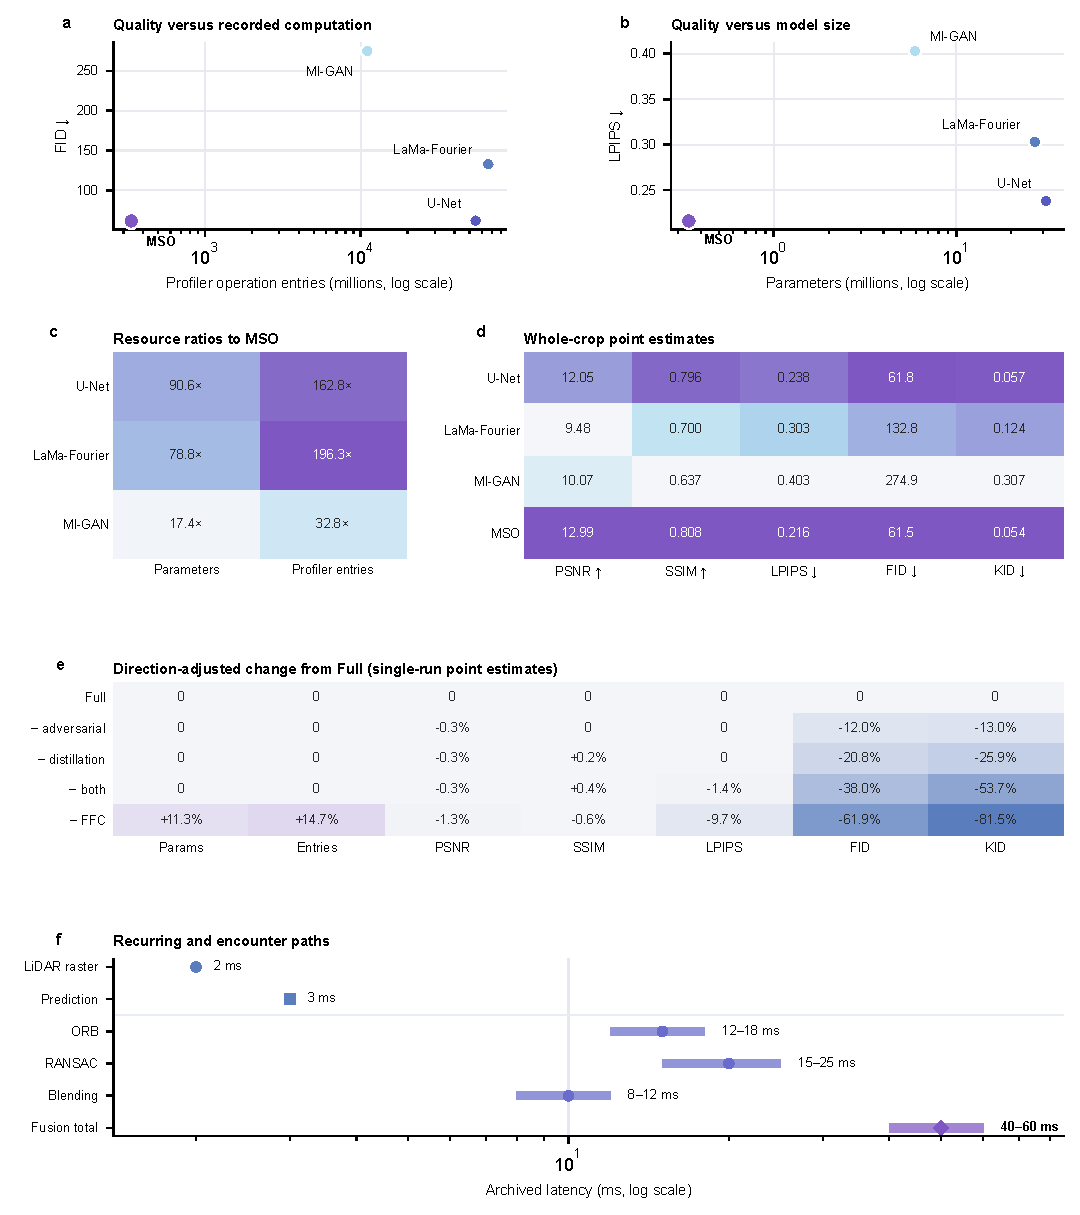
\includegraphics[width=\textwidth]{figure_resource_profile.pdf}
	\caption{\textbf{Resource and prediction profile.} \emph{a}, Archived profiler operation entries versus FID. \emph{b}, Parameter count versus LPIPS. Both horizontal axes are logarithmic, and lower values are favourable on both plotted dimensions. \emph{c}, Exact comparator-to-MSO ratios for parameters and profiler entries. \emph{d}, Raw whole-crop PSNR, SSIM, LPIPS, FID and KID point estimates. Colour is normalised within each metric only as a visual guide; annotations are the untransformed values. Observed cells comprise 51.1\% of pixels on average and are copied unchanged. \emph{e}, Direction-adjusted percentage changes from the full predictor across parameters, profiler entries and five quality metrics. Positive values indicate a favourable direction and negative values indicate an adverse direction. \emph{f}, Archived latency points and ranges. Markers identify CPU (circle), GPU (square) and mixed execution (diamond); rasterisation is per planner tick and prediction approximately 1 Hz. Ranges are operational, not statistical, and are not summed to reconstruct the separately reported total. Predictor values come from one retained training run per method or variant, so no training-seed uncertainty is shown.}
	\label{fig:resource-profile}
\end{figure}

\begin{table}[!htbp]
	\centering
	\caption{\textbf{Map fusion comparison on predicted, observed and simulated maps.} Success rate (SR) denotes the fraction of pairs whose post-registration Dice exceeds 0.83. Legacy RMSE, SSIM and Dice are descriptive post-warp summaries over all pairs; they do not directly measure relative-pose error. The archived source does not preserve the raster scaling used for RMSE, so its unitless values support within-table description only.}
	\label{tab:fusion-results}
	\MSOTableSetup
	\begin{tabularx}{\textwidth}{@{}l>{\raggedright\arraybackslash}Xrrrr@{}}
		\toprule
		\rowcolor{TableHeader}
		\textbf{Map} & \textbf{Algorithm} & \shortstack{\textbf{SR}\\$\uparrow$} & \shortstack{\textbf{Legacy RMSE}\\$\downarrow$} & \shortstack{\textbf{SSIM}\\$\uparrow$} & \shortstack{\textbf{Dice}\\$\uparrow$} \\
		\midrule
		Predicted & Ours (ORB-improved) & 0.125 & 0.797 & 0.944 & 0.588 \\
		          & ORB                 & 0.117 & 0.849 & 0.947 & 0.510 \\
		          & ICP                 & 0.000          & 1.063          & 0.920          & 0.448 \\
		\midrule
		Observed  & Ours (ORB-improved) & 0.059 & 0.765 & 0.978 & 0.579 \\
		          & ORB                 & 0.042          & 0.857          & 0.974          & 0.533 \\
		          & ICP                 & 0.000          & 1.171          & 0.960          & 0.326 \\
		\midrule
		Simulated & Ours (ORB-improved) & 0.844 & 0.347 & 0.970 & 0.911 \\
		          & ORB                 & 0.799          & 0.412          & 0.961          & 0.883 \\
		          & ICP                 & 0.001          & 0.967          & 0.891          & 0.575 \\
		\bottomrule
	\end{tabularx}
\end{table}

\begin{figure}[htbp]
	\centering
	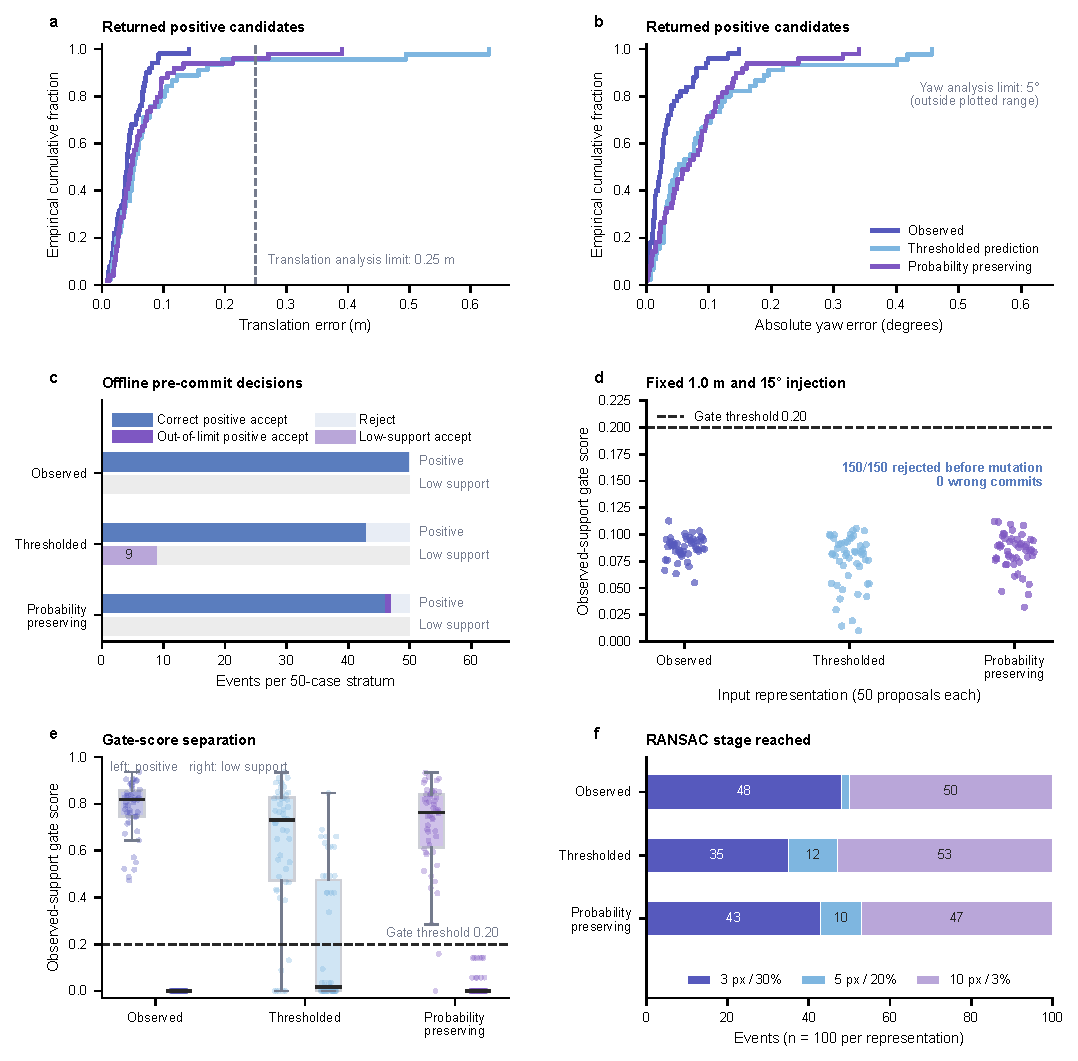
\includegraphics[width=\textwidth]{figure_transform_audit.pdf}
	\caption{\textbf{Controlled offline relative-pose and pre-commit acceptance audit.} \emph{a,b}, Empirical cumulative distributions of translation and absolute yaw error for rigid-valid candidates from positive encounters; dashed markers denote the analysis limits. \emph{c}, Pre-commit outcomes for 50 positive and 50 predeclared low-support events per representation; low-support events have no unique pose-error label. \emph{d}, Scores for 150 fixed-error proposals, all rejected below the 0.20 gate before simulated mutation. \emph{e}, Event-level scores for positive (left) and low-support (right) strata; points show events and boxes show median, interquartile range and 1.5-interquartile-range whiskers. \emph{f}, Events reaching each staged-RANSAC configuration. This single-scene audit uses a reconstructed reference implementation, not the deployed executable. Detailed values are in Supplementary Table~6 and the source-data archive.}
	\label{fig:transform-audit}
\end{figure}

\begin{figure}[htbp]
	\centering
	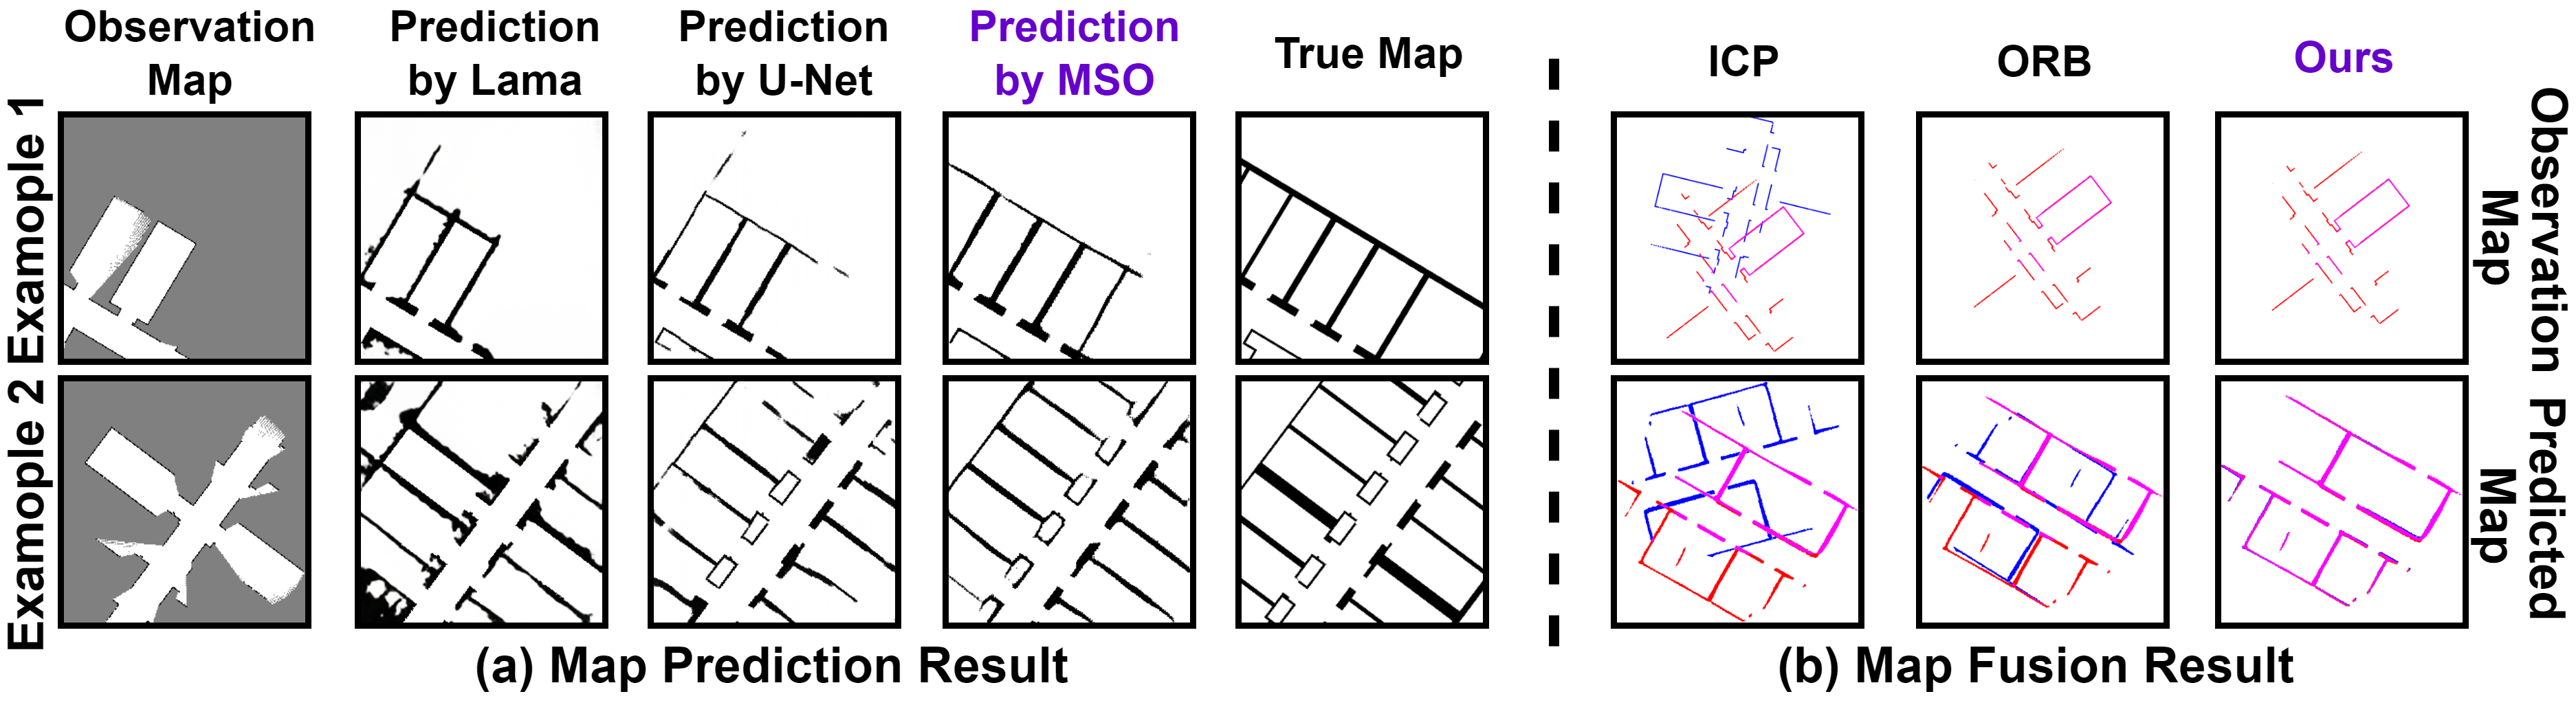
\includegraphics[width=\textwidth]{figure3.png}
	\caption{
		\textbf{Qualitative local map prediction and predictive map fusion results.}
		\emph{(a)} Two local-completion examples, one per row. Columns from left to right are partial observation, LaMa-Fourier, U-Net, MSO, and ground truth; grey marks unobserved cells and black marks obstacles.
		\emph{(b)} Two registration examples, one per row, shown for the tested ICP, ORB, and ORB-improved configurations. Red and blue denote the two inputs and magenta their rendered overlap. These cases illustrate the visual convention only; no ground-truth transform is overlaid, and quantitative overlap results are in Table~\ref{tab:fusion-results}.
	}
	\label{fig:map-results}
	\vspace{-0.67em}
\end{figure}
\subsection{Direct evaluation of predictive map registration} \label{sec:map-fusion-experiments}

\paragraph{Setting and baselines.}
We evaluate fusion on all 1{,}356 held-out samples (resized to $640{\times}640$) and the first 1{,}000 simulated pairs, comparing classical ORB~\citep{rublee2011orb} and ICP. We report success rate, legacy RMSE, SSIM and Dice ($>0.83$ is success). The source record does not preserve the raster scaling behind RMSE or the coordinate convention behind two additional distance summaries. We therefore treat RMSE as a unitless within-table descriptor, omit the two distances and use the controlled two-dimensional rigid-body-group SE(2) stress test for pose error. Both protocols are detailed in Methods.

\paragraph{Overlap results.} For the evaluated configurations, reported mean Dice on predicted maps is 0.588 for ORB-improved and 0.510 for ORB, while legacy RMSE is 0.797 and 0.849, respectively (Table~\ref{tab:fusion-results}). No paired interval is available, and these post-warp metrics do not directly measure pose correctness. The strict Dice$>$0.83 criterion is met by 0.125 of predicted-map pairs and 0.059 of observed-map pairs. Classical ORB has slightly higher SSIM on predicted maps (0.947 versus 0.944). The tested ICP configuration returns no successful predicted- or observed-map pair under this threshold; this result is specific to the reported parametrisation and is not evidence that ICP generally cannot register occupancy maps. Dice$>$0.83 remains an offline post-warp label and is not used as an acceptance rule.

\paragraph{Direct transform correctness and selective reliability.}
For this audit, a \emph{candidate} is a returned transform, an \emph{acceptance} is the gate decision before any persistent state change, a \emph{commit} would mutate persistent map or planner state, and \emph{recovery} would require detecting and reversing or otherwise clearing an incorrect committed mutation. The controlled experiments below evaluate candidates and offline pre-commit decisions; they do not execute commits or test recovery.
In the controlled offline stress test, the probability-preserving predicted-grid input gives median translation and yaw errors of 0.047\,m (95\% base-frame-cluster bootstrap interval 0.037--0.062\,m) and 0.066$^{\circ}$ (0.043--0.089$^{\circ}$), with P90 values of 0.108\,m and 0.146$^{\circ}$ (Fig.~\ref{fig:transform-audit}a,b; Supplementary Table~6). Under the 0.25\,m and 5$^{\circ}$ analysis tolerances, the offline pre-commit acceptance gate accepts 47 and rejects 53 of its 100 positive and \mbox{low-support} events: 46 positives are accepted within both limits, one accepted positive lies outside the translation limit, three positives are rejected, and all 50 predeclared \mbox{low-support} cases are rejected. The separately evaluated thresholded-prediction set accepts 43 positives within both limits, rejects seven positives, and accepts 9 of 50 \mbox{low-support} cases. Observed occupancy gives the lowest median errors, accepts all 50 positives within both limits, and rejects all 50 \mbox{low-support} cases in its selected set; the audit therefore does not show that predicted grids improve registration over observed maps. These are scene-limited, correlated offline events rather than independent buildings or online robot encounters, and a zero count is not interpreted as zero population risk. Acceptance is an offline decision before any commit and is not evidence that persistent robot state was updated.
The event-level score distributions and stage counts are exposed in Fig.~\ref{fig:transform-audit}e,f: among 100 events per representation, the loosest 10-pixel/3\% RANSAC stage is reached by 50 observed, 53 thresholded-prediction and 47 probability-preserving events. These counts describe the reconstructed audit path and are not a comparison of deployed computational cost.

\paragraph{Offline pre-commit rejection under erroneous proposals.}
We separately inject a fixed 1.0\,m and 15$^{\circ}$ error into 150 positive proposals. The ground-truth-free observed-support gate rejects all 150 before the harness's simulated atomic OR-merge; the harness target-mask hash remains unchanged and the changed-cell count is zero for every rejection (Fig.~\ref{fig:transform-audit}d; Supplementary Table~6). Feature matching is bypassed in this test. The result characterises the offline harness at the injected error level only and does not establish deployed commit behaviour, rollback or recovery.

\paragraph{Offline replay of the legacy deployment path.}
We also replay the recovered 2025 deployment source on ten archived two-robot bags. The replay exactly reproduces 1{,}325 of 1{,}485 recorded merged-map publications (89.2\%), but the bags contain neither transform nor acceptance-decision topics. Raster equality therefore cross-checks the replayed output without establishing transform correctness. The legacy partial-affine path does not enforce a proper unit-scale SE(2) model. Among exactly reproduced publications, 1{,}263 of 1{,}325 associated candidates fail the near-unit SE(2) structural test, and none passes structure together with the 0.25\,m and 5$^{\circ}$ diagnostic. A frozen counterfactual rigid estimator and gate return eight offline pre-commit acceptances among 1{,}644 cached-map callbacks; none satisfy the 0.25\,m and 5$^{\circ}$ limits, and two satisfy 0.50\,m and 10$^{\circ}$. Persistent-state commit remains disabled, giving zero recommended commits. This gate was not deployed, and the bag set cannot establish online relative-pose reliability, encounter-level false-accept or false-reject rates, rollback, or recovery.




\subsection{System-level exploration in simulation} \label{sec:exploration-efficiency}

\paragraph{Setting and baselines.}
We use one large indoor scene from MRPB~1.0, a unified benchmark for mobile-robot local planning~\citep{wen2021mrpb}. The predictor, trained on KTH and HouseExpo, was evaluated without reported fine-tuning. Coverage is the fraction of the ground-truth region physically observed. For reported occupied support $\widetilde O_t$ and ground truth $O_E$ in the same registered region,
\[
P_{\mathrm{occ}}(t)=|\widetilde O_t\cap O_E|/|\widetilde O_t|.
\]
This precision-like score does not penalise missed obstacles and is not IoU; nor does it measure free-space error, completion, topology, localisation or safety. The retained CSVs contain only the reported metric value, not its numerator and denominator, so the historical zero-denominator branch cannot be audited. The identically zero precision field for one nearest-frontier configuration is treated as an unavailable sentinel and omitted, not interpreted as measured zero precision. We interpret only retained numeric series and make no claim for an empty $\widetilde O_t$. All methods share the same initialisation, speed and LiDAR range; single robots predict within $2l$, and multirobot agents exchange maps within $4l$.

\paragraph{Results.} Fig.~\ref{fig:exploration-overview} provides four views of MRPB exploration. Two qualitative blocks show multirobot progression for frontier-multi, MSO-without-merge and full MSO, and the analogous single-robot comparison against MapEx~\citep{ho2024mapex} and IG-Hector~\citep{shrestha2019learned}. The lower panels report coverage and $P_{\mathrm{occ}}$ over time directly from retained aggregate CSV rows. At step 1500, the CSVs record coverage of 0.705 for full MSO and 0.604 for MSO-without-merge. Run-level seed traces were not retained, so the separation is descriptive and its seed-level variability cannot be reconstructed. Near step 1500, the retained single-robot aggregate trace is higher than the corresponding MapEx and IG-Hector traces; this comparison is also descriptive. The point estimates motivate the configuration used in the controlled physical trials; they do not constitute a matched comparison with PIPE, recent predictive multirobot approaches or graph-based collaborative-SLAM systems.

\begin{figure}[htbp]
	\centering
	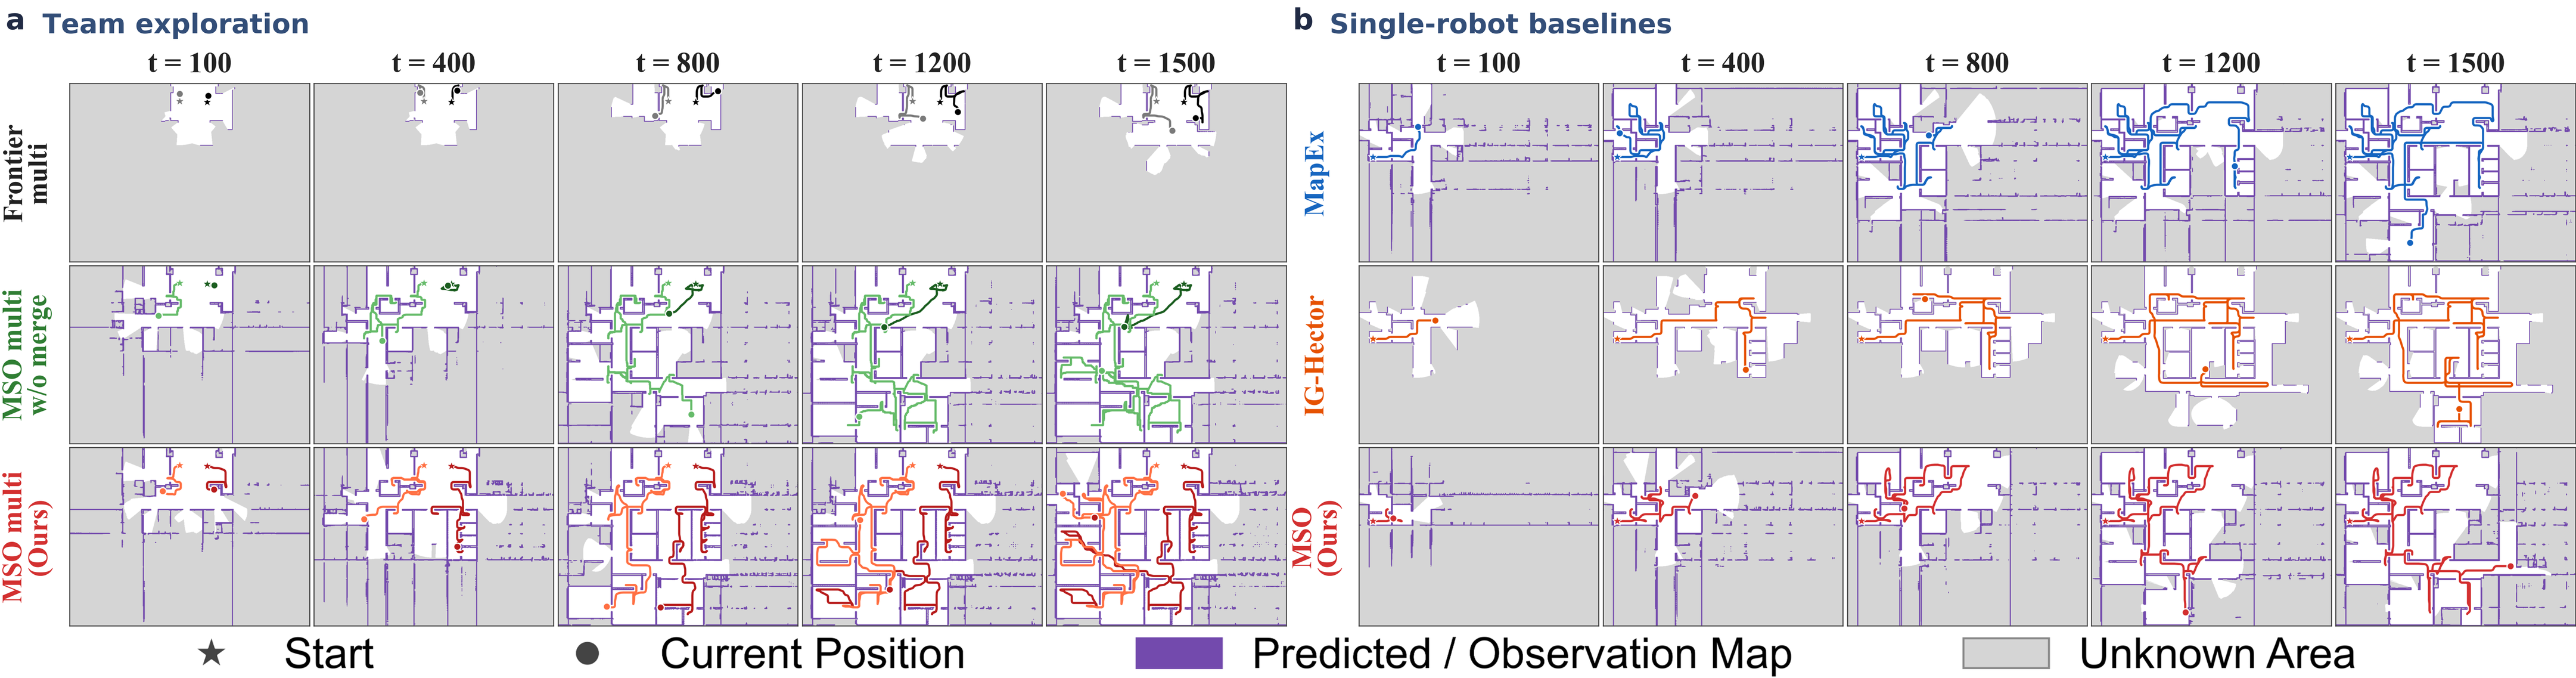
\includegraphics[width=\textwidth]{figure4_qualitative.png}\\[0.15em]
	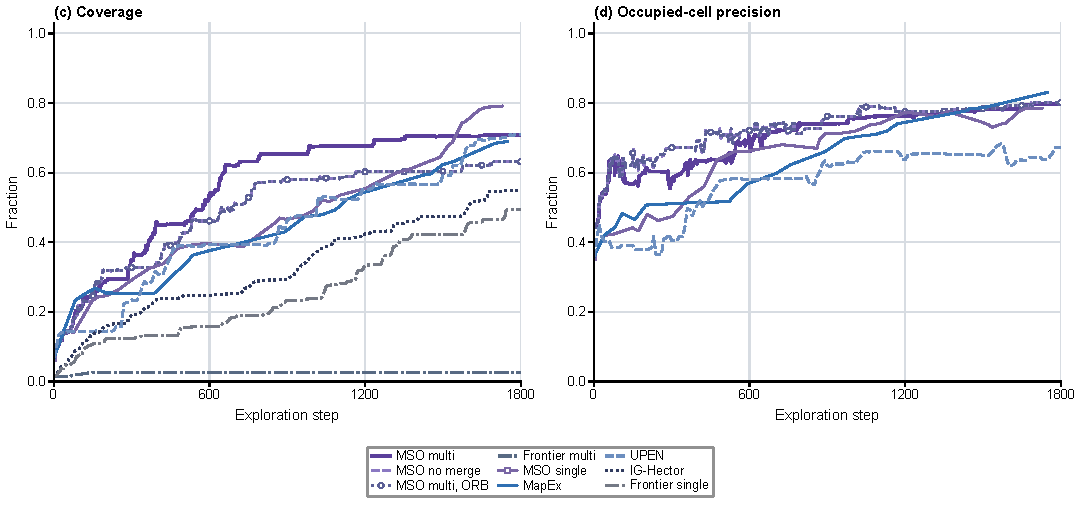
\includegraphics[width=\textwidth]{peer_review_data/mrpb/figs/fig5_exploration.pdf}
	\caption{\textbf{MRPB exploration and frame-by-frame progression.}
		\emph{a}, Multirobot progression at $t{=}100,400,800,1200,1500$ for frontier-multi, MSO-without-merge and full MSO. \emph{b}, Single-robot progression for MapEx, IG-Hector and MSO. \emph{c}, All nine retained coverage records. \emph{d}, Six occupied-cell-precision records from configurations with predictive completion outputs. Panels c and d plot every retained aggregate CSV row through step 1800 without interpolation or smoothing. The classical-ORB multirobot and no-merge records are identical over the displayed horizon; line style and sparse markers expose their overlap without offsetting the data. Precision fields from observed-only configurations, including the all-zero frontier-multirobot sentinel, are omitted rather than interpreted as prediction quality. Run-level seed traces were not retained, so per-seed variation and uncertainty intervals cannot be reconstructed.
		Within the qualitative panels, white is observed-free, light gray is uncertain, purple lines denote the \emph{Predicted Map} (observed plus predicted obstacles); trajectories use solid lines with $\star$/$\bullet$ at start/current, and the darker shade denotes robot~0.}
	\label{fig:exploration-overview}
\end{figure}
\begin{figure}[htbp]
	\centering
	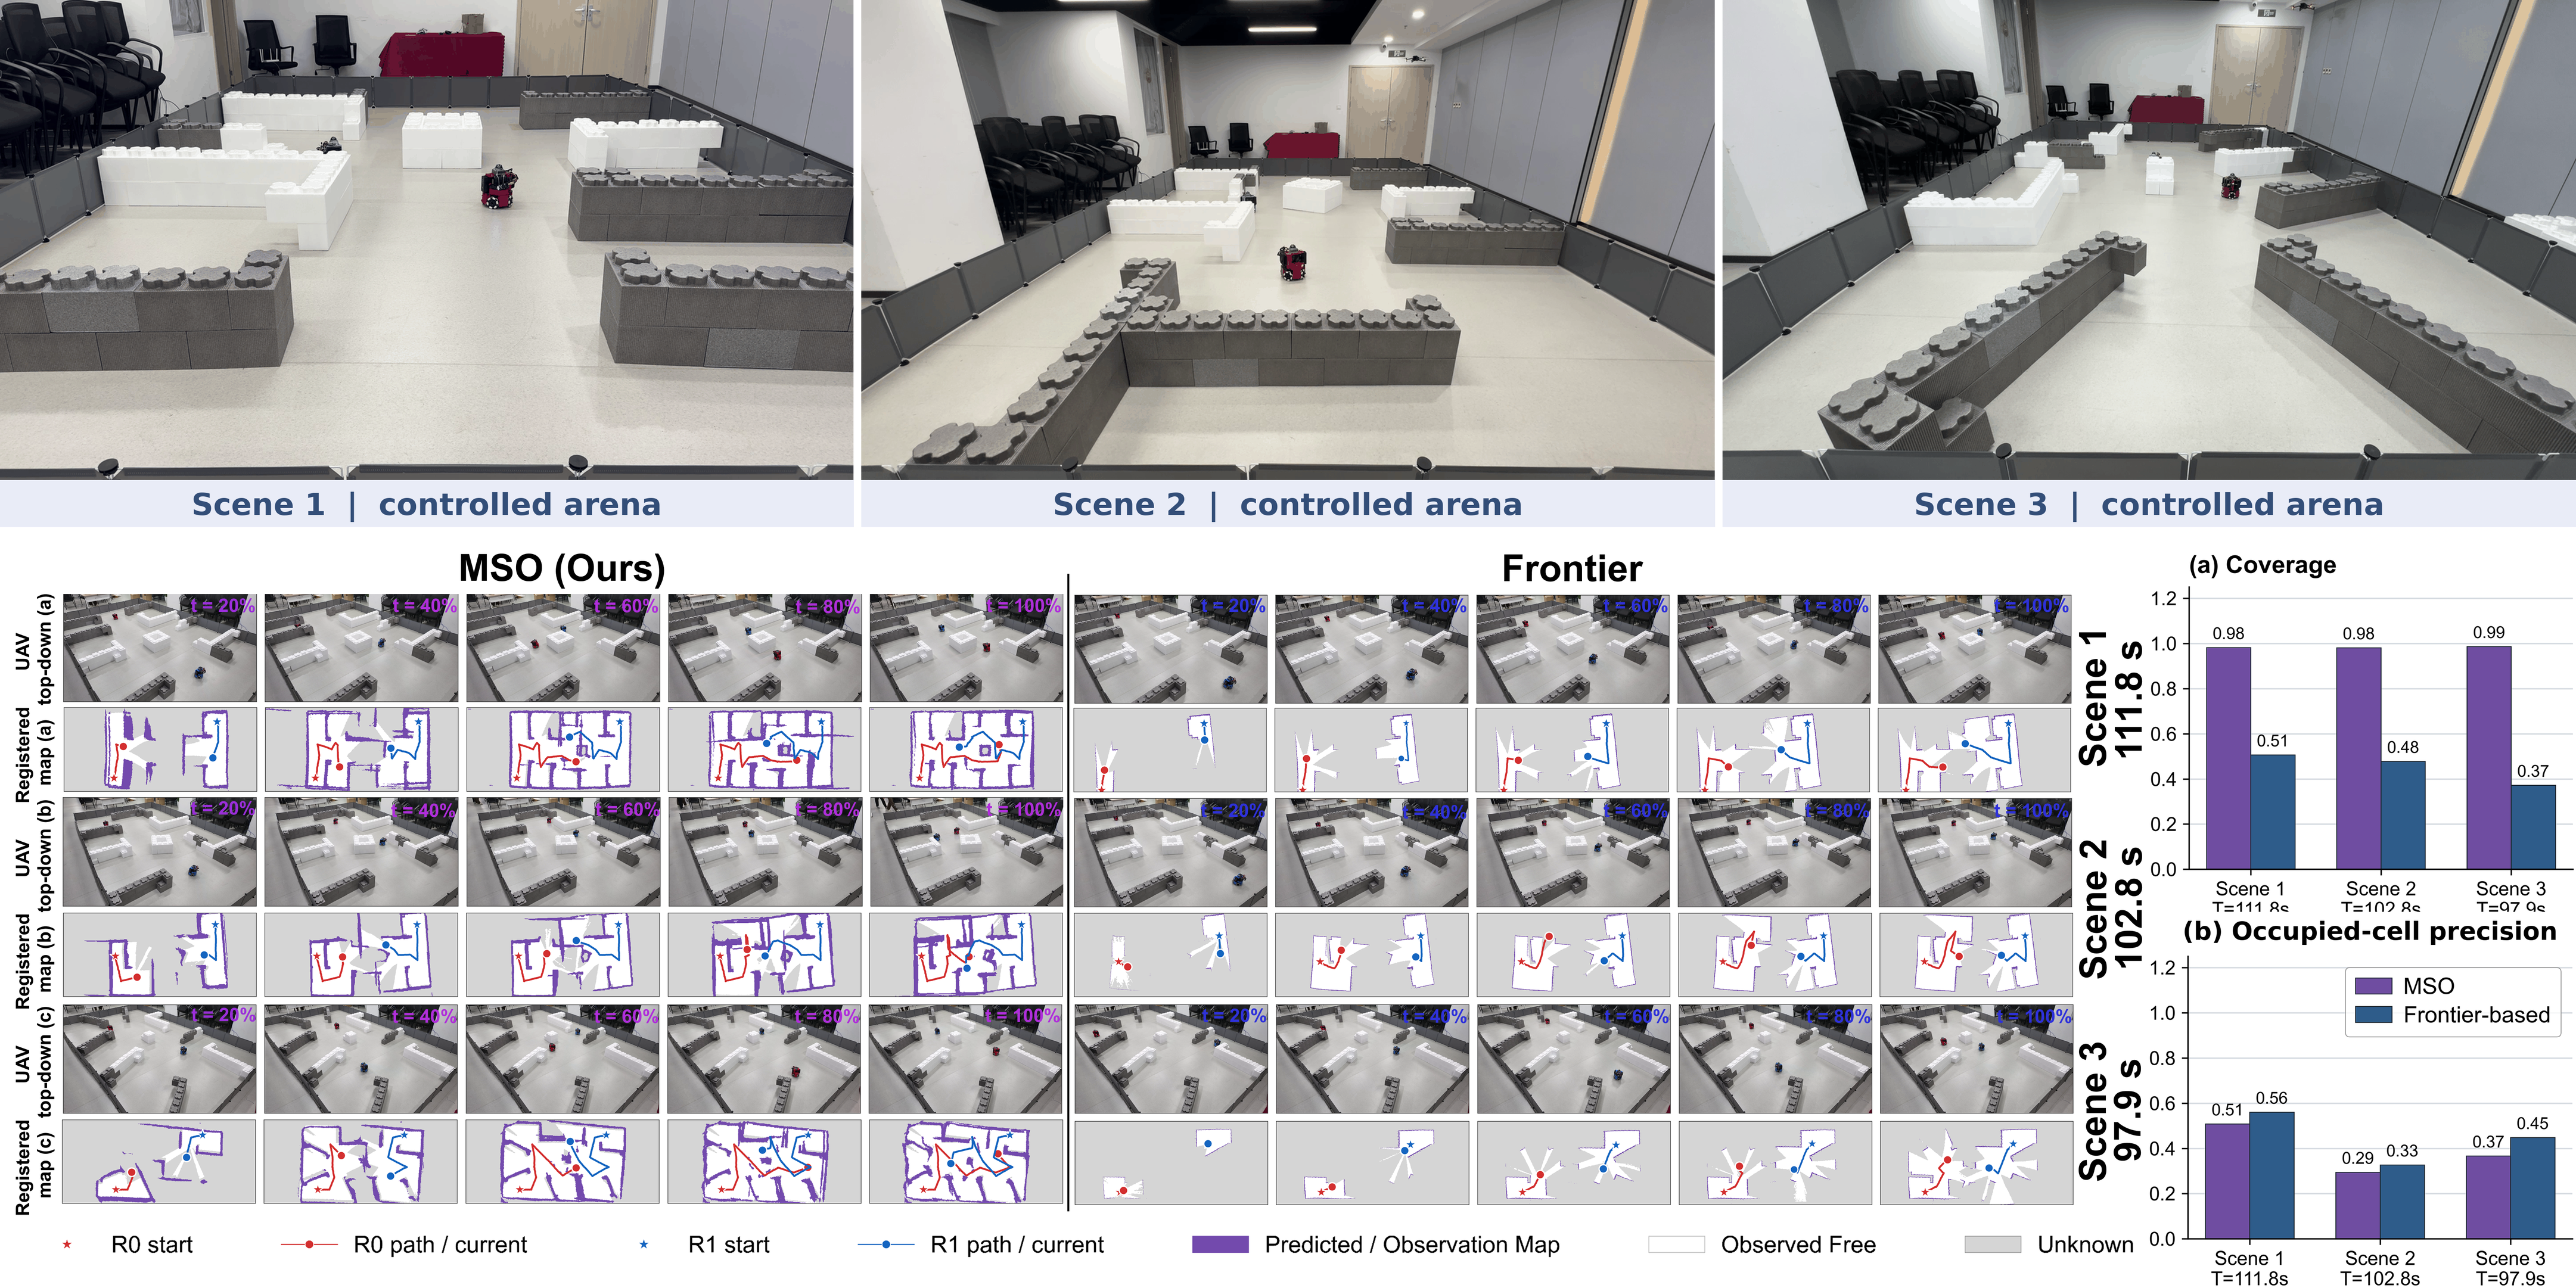
\includegraphics[width=\textwidth]{figure5_composite.png}
	\caption{\textbf{Descriptive two-robot results in controlled arenas.} Top, one mid-trial view of each $6.75\,\mathrm{m}\times4.05\,\mathrm{m}$ foam-block arena; these images document geometry and are not independent quantitative trials. Bottom, one legacy-path MSO run and one frontier-baseline run for each scene. Overhead images and offline UAV-referenced map visualisations show progress at 20--100\% of a run. Red and blue mark the two robots, and purple denotes predicted occupancy for MSO or observed obstacles for the frontier baseline. Bars report final coverage and occupied-cell precision $P_{\mathrm{occ}}$ under common sensing and motion settings. The displayed $T$ labels are MSO run durations; frontier durations were not retained, so the endpoints are not duration-matched. The offline visualisation is not evidence of deployed registration reliability or operation of the proposed gate.}
	\label{fig:real-world-results}
\end{figure}


\subsection{Legacy-path operation in controlled arenas} \label{sec:real-world-deployment}

Two self-built mobile robots (Livox Mid-360 LiDAR projected to a two-dimensional occupancy grid and an onboard Jetson computer) were recorded in three controlled $6.75{\times}4.05$\,m indoor arenas (Fig.~\ref{fig1}(c)). For each scene, Fig.~\ref{fig:real-world-results} reports one legacy-path MSO run and one frontier-baseline run under common $l{=}2$\,m, $v{=}0.5$\,m/s and start-pose protocol. The proposed rigid gate was not deployed in these runs. The prediction radius is 4\,m and communication radius is 8\,m. Because 8\,m exceeds the approximately 7.87\,m arena diagonal, the runs are effectively always connected and do not test disconnection, reconnection or leader turnover. All archived physical bags contain only robot~0 and robot~1. The $N{=}3$ and $N{=}5$ evidence is simulation-only. These runs are bounded demonstrations of the legacy deployment, not replicated estimates of the proposed architecture, physical-world performance or team scaling.

\paragraph{Results.} In Scenes 1, 2 and 3, the legacy-path MSO runs end at coverage 0.981, 0.980 and 0.986 after 111.8, 102.8 and 97.9\,s, respectively. The corresponding frontier runs end at coverage 0.506, 0.478 and 0.371 (Fig.~\ref{fig:real-world-results}). Frontier durations were not retained in the summary record, and stopping behaviour differs, so no duration-normalised comparison is made. MSO's occupied-cell precision is lower in each pair: 0.508 versus 0.560, 0.294 versus 0.327 and 0.366 versus 0.448. This metric does not measure missed obstacles, free-space error, completion, localisation or safety. The paired endpoint view in Fig.~\ref{fig:scaling-scene}f exposes the coverage--precision trade-off. With one run per scene and method, the values demonstrate bounded operation only.

\paragraph{Auxiliary single-robot archive.} Supplementary Fig.~5 restores the archived MSO, MapEx, UPEN and IG-Hector diagnostic on the same robot and arena. Its legacy ``explored free area'' label is the unmasked free-cell count over the complete \texttt{/map} raster multiplied by cell area, not region-of-interest-clipped arena coverage. MSO, MapEx and UPEN each have two included runs; IG-Hector has one because a failed run was excluded. Together with planner-specific stopping, this makes the display provenance evidence rather than a matched efficacy comparison.

\subsection{Fusion component ablation} \label{sec:fusion-component-results}

\begin{table}[!htbp]
	\centering
	\caption{\textbf{Fusion component ablation on the predicted-map split.} We report success rate (Dice$>0.83$), mean Dice, legacy unitless RMSE and SSIM. Values are descriptive point estimates on matched inputs; no typographic emphasis or inferential ranking is intended.}
	\label{tab:fusion-ablation}
	\MSOTableSetup
	\begin{tabular*}{\textwidth}{@{\extracolsep{\fill}}lcccc@{}}
			\toprule
			\rowcolor{TableHeader}
			\textbf{Variant}                          & \textbf{Success rate} $\uparrow$ & \textbf{Dice} $\uparrow$ & \textbf{Legacy RMSE} $\downarrow$ & \textbf{SSIM} $\uparrow$ \\
			\midrule
			Full (ORB-improved)                       & 0.125                            & 0.588                    & 0.797                       & 0.944                    \\
			w/o ambiguity-heuristic weighting         & 0.118                            & 0.534                    & 0.831                      & 0.942                    \\
			w/o multi-scale                           & 0.121                            & 0.572                    & 0.842                      & 0.934                    \\
			w/o staged RANSAC                         & 0.106                            & 0.575                    & 0.819                      & 0.941                    \\
			\bottomrule
	\end{tabular*}
\end{table}

Disabling ambiguity-heuristic weighting changes Dice from $0.588$ to $0.534$. Removing the $0.5{\times}$ and $0.25{\times}$ feature pools changes legacy RMSE from $0.797$ to $0.842$ and SSIM from $0.944$ to $0.934$. Replacing staged RANSAC with one relaxed pass changes the strict success rate from $0.125$ to $0.106$. No uncertainty interval or hypothesis test is available, so these point differences are not interpreted as statistically established rankings.
The conference draft also reported a 200-clip streaming temporal-prior row. Its source record was not recovered, so that row is disclosed here but omitted from the quantitative table rather than reconstructed from the earlier typeset values alone.

\subsection{Generalisation and scaling boundaries} \label{app:scaling}

\paragraph{Simulated team size.}
We assess retained aggregate coverage traces for full MSO from a separate auxiliary MRPB campaign with $N\!\in\!\{2,3,5\}$ robots. The experiments were configured for five random seeds per team size, but run-level seed files and the campaign manifest were not retained; the traces are therefore treated descriptively and do not support seed-level uncertainty estimates. They use their native logged-step axis and end at their recorded termination points rather than the main experiment's fixed 1500-step horizon. The available records do not establish that the auxiliary $N{=}2$ trace and the main full-MSO trace share the same initialisation, step definition, aggregation rule or software revision. They are not compared numerically, and the auxiliary curves are not interpreted as a controlled team-size effect or as latency, memory or communication scaling.

The retained traces terminate at recorded steps 387, 221, and 96 for $N{=}2,3,5$, with final coverages of 0.839, 0.835, and 0.943, respectively (Fig.~\ref{fig:scaling-scene}a--c; Supplementary Fig.~1). Because the endpoints differ in coverage and the run-level provenance is incomplete, their ratios are not interpreted as matched-coverage speed-ups. For source-record description only, the first logged steps at which coverage is at least 0.8 are 79, 82, and 24 for $N{=}2,3,5$, respectively.

\paragraph{In-distribution KTH floorplan.}
We report the retained aggregate coverage trace for full MSO (\texttt{ours\_multi\_ours\_orb}) on one KTH scene reported as held out at floorplan level. The experiment was configured for five random seeds, but run-level seed files were not retained. KTH layouts contribute to the predictor's reported training data, while the exact historical split manifest needed to verify this floorplan assignment was not recovered.

The retained full-MSO coverage trace ends at 0.951 (Fig.~\ref{fig:scaling-scene}d,e; Supplementary Fig.~2). No machine-readable KTH occupied-cell-precision series was retained, so that quantity is not plotted or inferred. This is a one-floorplan descriptive result from the reported KTH partition rather than an independently verified test of floorplan- or building-level transfer.

\begin{figure}[htbp]
	\centering
	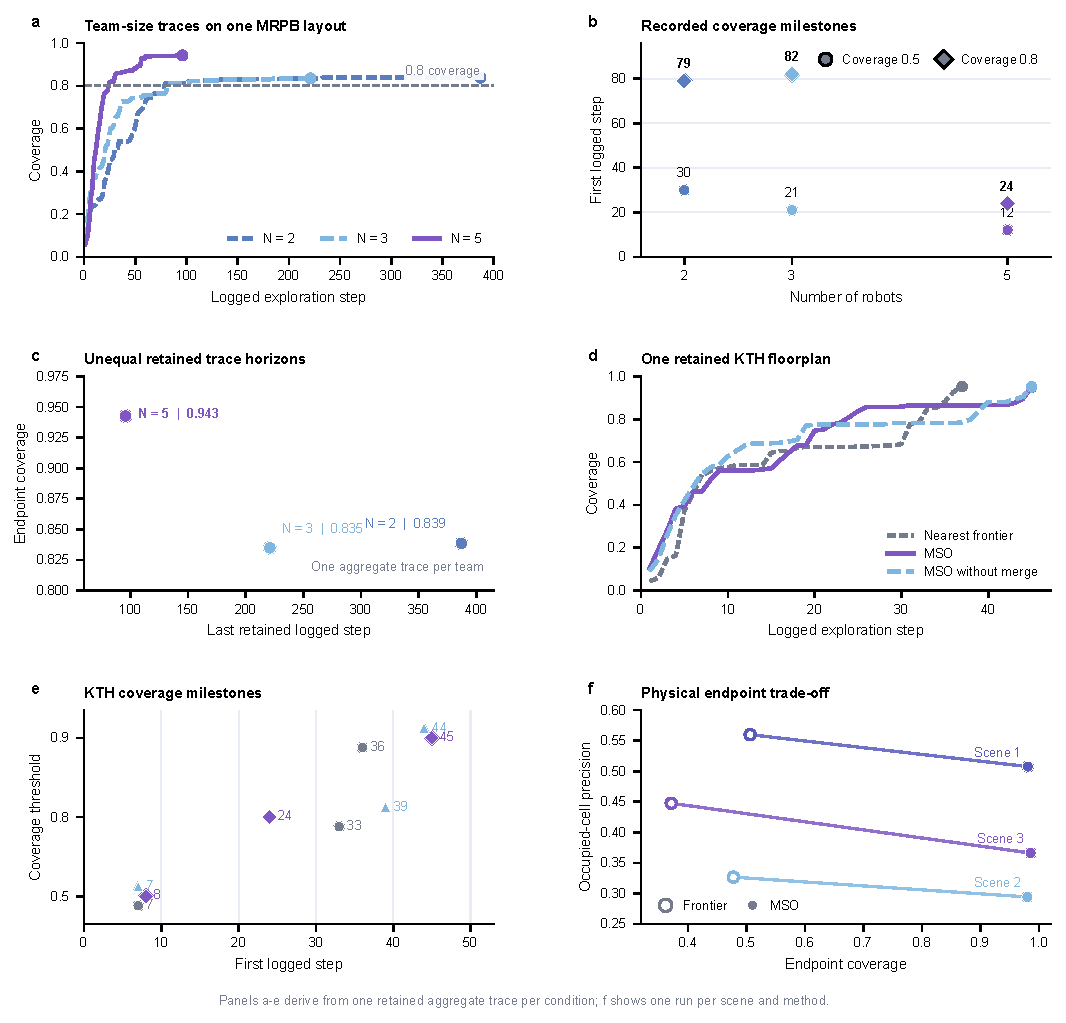
\includegraphics[width=\textwidth]{figure_scaling_scene.pdf}
	\caption{\textbf{Retained system-level traces and physical endpoint trade-off.} \emph{a}, Coverage over the native logged-step axis for $N{=}2,3,5$ robots in a separate auxiliary MRPB campaign. \emph{b}, First logged steps at which each trace reaches coverage 0.5 and 0.8. \emph{c}, Final coverage plotted against the last retained logged step, exposing the unequal trace horizons. These values describe the retained files and are not a controlled team-size effect. \emph{d}, Coverage for full MSO, MSO without merge and a nearest-frontier configuration on one KTH floorplan reported as held out. \emph{e}, First logged steps at which the three KTH traces reach coverage 0.5, 0.8 and 0.9; adjacent labels give the exact recorded steps. \emph{f}, Coverage and occupied-cell precision for one MSO and one frontier run in each physical scene; lines connect runs within a scene and do not denote a sampled trajectory. Panels a--e derive from one retained aggregate trace per condition from experiments configured for five seeds, but run-level records were not retained. No seed-level uncertainty is shown, differing endpoints are not interpreted as matched-horizon speed-ups, and panel f is descriptive. Source data are provided with the accompanying archive.}
	\label{fig:scaling-scene}
\end{figure}

\paragraph{Completion failure modes.}
Supplementary Fig.~3 provides ten additional held-out completion examples. Two recurring failure modes remain. When a local field of view contains almost no wall geometry, MSO occasionally hallucinates a faint short partition near the boundary of the uncertain region. In scenes dominated by long, thin diagonal walls, which are rare in the KTH/HouseExpo training distribution, MSO sometimes splits the wall into short orthogonal segments aligned with dominant training axes. These examples are qualitative and do not replace topology- or navigation-specific metrics.

%===============================================================================

\section{Discussion} \label{sec:discussion}
The principal contribution of MSO is a resource-constrained architecture and retrospective audit for connecting learned prediction, relative-map alignment and observation-constrained planning. The design is governed by three contracts. A resource contract bounds prediction and fusion computation. A geometric contract separates transform proposal from offline pre-commit acceptance. A mapping-authority contract allows predicted structure to guide alignment and frontier ranking while measured occupancy remains authoritative for collision checking and persistent-map updates. The preserved records test parts of these contracts through model size, transform error, offline acceptance outcomes, harness state hashes, exploration coverage and occupied-cell precision. They do not validate all contracts in one deployed implementation.

The component evaluations expose both capability and trade-off. The compact predictor has favourable whole-crop point estimates relative to the evaluated larger inpainting backbones, but copied observed pixels contribute to those metrics and single training runs do not establish the stability of their ordering. In the selected offline pose test, probability-preserving prediction produces small median errors and one out-of-limit accepted positive, whereas observed occupancy yields lower median errors; the test does not demonstrate a registration advantage from prediction. In the physical study, the recorded legacy-path MSO runs have higher endpoint coverage and lower occupied-cell precision than their corresponding frontier runs. Because there is only one run per method and scene, stopping behaviour differs, frontier durations are unavailable and trial order was not randomised, those pairs provide bounded operation examples rather than a comparative treatment estimate.

The ambiguity and acceptance evidence is similarly bounded. The Bernoulli score is a deterministic, low-cost ambiguity heuristic rather than calibrated epistemic uncertainty. The direct transform audit uses selected moderate-overlap snapshots from one scene and a reference implementation reconstructed from the specification, not the deployed executable. The wrong-transform experiment bypasses feature matching; it shows that, for one fixed injected error, rejected proposals do not mutate the harness target mask before a simulated atomic OR-merge. The separate deployment-source replay reproduces many merged rasters but lacks recorded transforms and decisions. Its frozen rigid audit supports only a fail-closed, no-commit recommendation, not online correctness, rollback or recovery. These distinctions prevent either offline audit from being interpreted as deployed registration validation.

The historical experiment record reports floorplan separation between fitting and held-out crops, but the missing split manifest prevents independent verification. The principal exploration comparison uses one MRPB environment, the KTH result uses one floorplan from the reported partition, and the physical campaign uses two robots in small foam-block arenas whose communication radius exceeds the arena diagonal. No simultaneous three- or five-robot physical record was found. Within this operating envelope, the study provides separate component audits and bounded legacy-path demonstrations. It does not show the proposed registrar, gate, planner and persistent-state mutation operating together, establish a causal coverage improvement, or support building-level and physical-team generalisation. Closing these gaps requires one frozen end-to-end implementation, an auditable predictor split and checkpoint, common-horizon replicated trials, matched contemporary baselines, communication impairment and larger physical teams.

%===============================================================================

\section{Methods} \label{sec:methods}

\subsection{Map and agent model} \label{app:problem}

The environment is represented by a two-dimensional occupancy grid with fixed metric resolution and dynamic extent. Each map record contains a timestamp, resolution, origin and occupancy-probability array. The observation encoder uses \emph{Obstacle}, \emph{Uncertain} and \emph{Free} channels in that order; the predictor outputs occupied-cell probability on the uncertain region. Each robot maintains its own measured map $M_i$, localises within that map, plans collision-free paths on measured occupancy and communicates with peers inside a prescribed range. Initial pairwise transforms between robot maps are unknown. At a communication encounter, a candidate transform maps the peer grid into the temporary leader's frame; a proposal can be rejected before fusion. Predictions remain provisional and subsequent sensor measurements take precedence.

\subsection{Training objectives} \label{app:losses}

Let $x_{\text{obs}}\in\{0,1\}^{3\times H\times W}$ be the observed map with channels ordered \emph{Obstacle}, \emph{Uncertain} and \emph{Free}. Let $o_{\text{obs}}=x_{\text{obs}}^{(\mathrm{Obstacle})}\in\{0,1\}^{1\times H\times W}$ and $\textit{mask}=x_{\text{obs}}^{(\mathrm{Uncertain})}\in\{0,1\}^{1\times H\times W}$. The target $x_{\text{true}}\in\{0,1\}^{1\times H\times W}$ is a binary occupied-cell raster, and $x_{\text{pred}}=f_G(x_{\text{obs}})\in[0,1]^{1\times H\times W}$ is the predicted occupied-cell probability. Singleton channel dimensions are suppressed below; no three-to-one-channel broadcasting is used.

\paragraph{Adversarial loss.}
Following the masked discriminator design of Suvorov et al.~\citep{suvorov2021resolution}, we first form the completed map
\begin{equation}
	x_{\text{comp}}=(1-\textit{mask})\odot o_{\text{obs}}+\textit{mask}\odot x_{\text{pred}},
\end{equation}
so observed occupied cells are copied from $o_{\text{obs}}$ and observed free cells remain zero. With $D_m(x)$ the discriminator response after concatenating the one-channel raster $x$ and one-channel mask along the channel dimension, averaged over patches intersecting the mask, the non-saturating losses are
\begin{equation}
	\begin{aligned}
		\mathcal{L}_{D} =
		-\mathbb{E}_{x_{\text{true}}}\!\left[\log D_m(x_{\text{true}})\right]
		-\mathbb{E}_{x_{\text{obs}},\textit{mask}}\!\left[\log\!\left(1-D_m(x_{\text{comp}})\right)\right],
	\end{aligned}
\end{equation}
\begin{equation}
	\mathcal{L}_{\text{Adv}}
	=
	\mathcal{L}_{G}^{\text{Adv}}
	=
	-\mathbb{E}_{x_{\text{obs}},\textit{mask}}\!\left[\log D_m(x_{\text{comp}})\right].
\end{equation}
The discriminator minimises $\mathcal{L}_D$ and each generator uses $\mathcal{L}_{\text{Adv}}$.

\paragraph{Feature-reconstruction loss.}
We align features from a high-receptive-field ResNet $\phi(\cdot)$ at layer $j$~\citep{chi2020fast,he2016deep}:
\begin{equation}
	\mathcal{L}_{\mathrm{feature}}=\frac{1}{C_j H_j W_j}\|\phi_{j}(x_{\mathrm{pred}})-\phi_{j}(x_{\mathrm{true}})\|^2_2 ,
\end{equation}
where $C_j,H_j,W_j$ are the feature dimensions. We omit the style loss~\citep{johnson2016perceptual}. The surviving record does not specify any channel replication or normalisation before $\phi$; this equation documents the reported objective rather than an independently executable historical loss module.

\paragraph{Masked $L_2$ loss.}
The masked pixel loss is
\begin{equation}
	\mathcal{L}_{L_2} = \frac{1}{\|\textit{mask}\|_1+\epsilon} \left\| (x_{\text{true}} - x_{\text{pred}}) \odot \textit{mask} \right\|_2^2 ,
\end{equation}
and penalises only \emph{Uncertain} pixels.

\paragraph{Teacher objective.}
The teacher minimises
\begin{equation}
	\mathcal{L}_{\text{Teacher}} = \alpha \mathcal{L}_{\text{Adv}} + \beta \mathcal{L}_{\mathrm{feature}} + \gamma \mathcal{L}_{L_2} .
\end{equation}

\paragraph{Distillation and student objective.}
For aligned layer $i$, the $1\times1$ projection $f_{\mathrm{point}}^{i}(\cdot)$ maps teacher channels onto student channels and gives
\nopagebreak[4]
\begin{equation}
	\mathcal{L}_{\mathrm{distill}}^i=\frac{1}{C^{i}_{\mathrm{Student}} H^i W^i}\|f_{\mathrm{point}}^i(f_{\mathrm{Teacher}}^i(x_{\mathrm{obs}}))-f_{\mathrm{Student}}^i(x_{\mathrm{obs}})\|_2 ,
\end{equation}
giving the overall student objective
\begin{equation}
	\mathcal{L}_{\text{Student}} = \alpha\mathcal{L}_{\text{Adv}} + \beta \mathcal{L}_{\text{feature}} + \gamma \mathcal{L}_{L_2} + \Lambda \sum_{i=1}^{N}\mathcal{L}_{\text{distill}}^i ,
\end{equation}
where $N=4$. The exact trainer, several loss modules, manuscript checkpoint, validation manifest and checkpoint-selection trace were not preserved; the reported image scores are therefore descriptive historical point estimates.

\paragraph{Architecture.}
The student is a five-resolution encoder--decoder for $256{\times}256{\times}3$ inputs, with widths $4\!\to\!8\!\to\!16\!\to\!32\!\to\!64$. It combines depthwise-separable convolutions, FFC residual blocks~\citep{suvorov2021resolution,chi2020fast}, skip connections and transposed-convolution upsampling. A sigmoid head returns an occupied-cell probability. The model has 342{,}771 trainable parameters. An archived static profile stores a scalar of 336.151 million operation entries at this input size; ``entry'' does not identify an elementary-operation convention. The profiler name/version, batch convention, graph precision and multiply--accumulate rule were not retained, and no warm-up or repeat distribution accompanies the count. It is therefore not labelled as MACs, FLOPs or latency. The teacher uses base width 32 and extra convolution/FFC blocks; four feature pairs are aligned by $1{\times}1$ projections. The FFC-augmented PatchGAN~\citep{isola2017image,suvorov2021resolution} scores patches intersecting the uncertain mask. Augmentation comprises horizontal/vertical flips and $90^{\circ}$ rotations.

\subsection{Map fusion pipeline} \label{app:fusion}

Predicted-map descriptors may lie on observed geometry or model-generated structure. MSO therefore uses prediction as a feature-rejection and correspondence-weighting heuristic before estimating a pairwise rigid transform. This is a registration front end, not pose-graph optimisation or a temporal transform model.

\paragraph{Multi-modal feature pool.}
At each scale, ORB keypoints $\mathcal{F}_{\text{ORB}}$, Canny-edge features $\mathcal{F}_{\text{Edge}}$ and morphological-skeleton features $\mathcal{F}_{\text{Morph}}$ capture complementary structure. Lower-resolution coordinates map to the full grid as $p_{\text{full}}=2^{k}p_{\text{low}}$. Each family applies $\mathcal{U}(k)<0.8\,\mathrm{mean}(\mathcal{U})$; matching additionally requires $w_m>0.5$ before RANSAC.

\paragraph{Encounter-level multi-resolution scheduling.}
At an encounter, robots elect a temporary leader, an implementation mechanism rather than a contribution. Peers extract three-scale features locally; the leader registers each peer and limits full-resolution refinement to the estimated overlap. Robots exchange odometry, predicted maps and event-driven sparse features (Supplementary Table~3). The 40--60\,ms timing and bandwidth audit describe two robots only; runtime, memory and traffic were not measured across team sizes.

\paragraph{Algorithm.}
Figure~\ref{fig2}b and Supplementary Algorithm~1 distinguish candidate generation, geometric filtering, offline pre-commit acceptance and simulated map mutation. The offline reference path and legacy deployed implementation are separate software artefacts.

\subsection{Fusion component ablation protocol} \label{app:fusion-ablation}
We re-run the predicted-map split (1{,}356 held-out pairs; Table~\ref{tab:fusion-results}) with one component removed and all other settings fixed:
\textbf{w/o ambiguity-heuristic weighting} sets $\mathcal{U}{=}1$ everywhere and disables both the keypoint pre-filter ($\mathcal{U}{<}0.8\,\overline{\mathcal{U}}$) and the match-weight $w_m$;
\textbf{w/o multi-scale} retains only the $1\times$ feature pool, removing the $0.5\times$ and $0.25\times$ pyramids and the cross-scale RANSAC voting;
\textbf{w/o staged RANSAC} replaces the progressive thresholds ($3.0/30\%{\to}5.0/20\%{\to}10.0/3\%$) by a single RANSAC pass at the relaxed final threshold.

\subsection{Dataset construction} \label{app:dataset}

We set $[\sigma_1,\sigma_2]=[1.5,8.0]$\,m, obstacle ratio $[\Phi_1,\Phi_2]=[0.05,0.45]$ and free ratio $[\Phi_3,\Phi_4]=[0.20,0.85]$. Each observation is a three-channel $256{\times}256$ tensor whose target is cropped from the global grid at the agent pose. The historical record reports exact-sample deduplication to 5{,}385 fitting and 1{,}356 held-out samples, averaging $39.4\%$ free, $11.7\%$ obstacle and $48.9\%$ uncertain pixels, with each parent floorplan confined to one partition. The sample manifest was not recovered. The closest archive instead has 6{,}841 train-labelled and 1{,}463 test-labelled samples, with no exact processed duplicate across labels but without consistent floorplan/building identifiers or an independent validation partition. It cannot reconstruct the manuscript split or exclude model-selection contact with the reported evaluation set. We therefore do not claim verified floorplan- or building-disjoint generalisation or a locked test set.

\subsection{Implementation training and evaluation setup} \label{app:training}

\paragraph{Training.} The historical record reports Adam ($\text{lr}{=}10^{-3}$, $\beta_1{=}0.5$, $\beta_2{=}0.999$), 500 epochs, one A100 GPU and batch size $16$ for teacher and student. Loss weights are $\alpha{=}10$, $\beta{=}30$, $\gamma{=}1$ and $\Lambda{=}5$ across $N{=}4$ student layers. The training entry is unavailable. Two recovered candidates load the 342{,}771-parameter student and record epoch 499 and step 72{,}000, but neither is identified as the manuscript checkpoint; their Adam state uses betas $(0.0,0.99)$, conflicting with the reported setting, so they do not revise manuscript results. U-Net, LaMa-Fourier and MI-GAN use their reported defaults except that the \emph{Uncertain} channel is the loss mask.

\paragraph{MRPB exploration setup.}
The experiment was configured for 50 random seeds per method on one MRPB scene~\citep{wen2021mrpb}, but only one aggregate trace per method was retained. Run-level seed files and time-resolved dispersion summaries are unavailable, so the full per-seed distribution and s.d. cannot be reconstructed and the curves are analysed descriptively. Methods share $0.5$\,m/s speed and LiDAR range $l$; single robots predict within $2l$ and multirobot agents exchange maps within $4l$. Occupied-cell precision is $P_{\mathrm{occ}}(t)=|\widetilde O_t\cap O_E|/|\widetilde O_t|$ in a common registered region. It is not IoU because false negatives do not enter the denominator, and it does not support completion or safety claims. Numerator and denominator counts were not retained, so the historical zero-denominator convention cannot be reconstructed; one identically zero sentinel field is treated as unavailable and excluded.

\paragraph{Map-fusion evaluation protocol.} \label{app:eval}
Each of 1{,}356 held-out pairs is resized to $640{\times}640$. Dice is computed over registered binary obstacle maps and Dice$>0.83$ denotes success, following prior work~\citep{ho2024mapex}. Legacy RMSE, SSIM and Dice are post-registration summaries over the common output raster. The archived evaluator does not preserve the raster scaling used for RMSE, so the reported values are unitless and interpreted only within the table. The simulated split additionally supplies ground-truth transforms. Two legacy matched-coordinate distance summaries are omitted because their coordinate convention and aggregation unit are also unresolved.

\paragraph{Direct-transform stress test.}\label{app:transform-correctness}
We separately construct an archived offline benchmark from the saved two-robot A3 map stream, whose grids share a $1020{\times}424$ raster at $0.05$\,m per pixel. This is a new controlled test rather than a relabelling of the 1{,}356/1{,}000-pair overlap experiment. For each of five fixed perturbation seeds (11, 23, 37, 53 and 71) and each of three inputs---observed occupancy, thresholded prediction and probability-preserving prediction---we select ten same-timestamp positive pairs whose occupied-support overlap coefficient is at least 0.30 when measured in the shared ground-truth raster before applying a perturbation. We then apply to the source a saved random translation of 0.25--1.50\,m and a saved random yaw of 5--30$^{\circ}$. Ten same-scene temporal mismatches per seed, separated by at least ten logged steps and with support IoU at most 0.05 in that shared raster, form predeclared low-support abstention cases. This gives 50 positives and 50 low-support cases per input representation. Selection, perturbations, labels and file hashes are fixed before running the registrar. The positives therefore represent selected moderate-overlap events, not the low-overlap extreme motivating predictive registration. Because all snapshots come from one scene, the test measures controlled pose recovery and abstention, not cross-building generalisation.

The archived reference implementation is reconstructed from the specification, not replayed from the deployed executable. Grayscale probabilities are divided by 255 and the ambiguity heuristic is zero on observed cells. Canny thresholds are 50/150; $3{\times}3$ cross-element skeletonisation runs for at most 32 passes; ORB budgets at $1{\times}$, $0.5{\times}$ and $0.25{\times}$ are 1100, 550 and 275. Edge/skeleton points use \texttt{goodFeaturesToTrack} (quality 0.005; four-pixel separation). Residual filters retain angle, log-scale and displacement within four scaled median absolute deviations, with floors of 45$^{\circ}$, $\log(1.8)$ and 160 pixels. Staged \texttt{estimateAffinePartial2D} uses confidence 0.99 and ten refinement iterations. These settings and the selected events accompany the event manifest.

Define $\mathbf{T}_{i\leftarrow j}\in\mathrm{SE}(2)$ from source $j$ to target $i$. For estimate $\widehat{\mathbf T}$ and saved perturbation inverse $\mathbf T^{\star}$, $\mathbf E=(\mathbf T^{\star})^{-1}\widehat{\mathbf T}$. Translation and yaw errors are $e_t=\|\operatorname{trans}(\mathbf E)\|_2$ and $e_{\psi}=|\operatorname{wrap}(\operatorname{atan2}(E_{21},E_{11}))|$; analysis limits are 0.25\,m and 5$^{\circ}$. Without reading ground truth, the offline pre-commit acceptance gate requires positive determinant, both singular values within 0.02 of one, RANSAC inlier ratio at least 0.20 and observed occupied-support overlap at least 0.20 after warping. Predicted inputs are checked against companion observed grids, so generated structure alone cannot authorise acceptance. Accepted affines are projected to the nearest rotation while retaining translation; invalid candidates are rejected.

Let $A$ denote an offline pre-commit acceptance, $P$ a positive encounter and $C$ a positive whose transform is within both analysis limits. For positives, Fig.~\ref{fig:transform-audit}c and Supplementary Table~6 report $A\cap C$ as a correct accept, $A\cap\neg C$ as an out-of-limit accept, and $\neg A\cap P$ as a positive reject. The low-support temporal-mismatch cases do not have a unique ground-truth transform and are predeclared abstention challenges; their accepted and rejected counts are reported separately rather than interpreted as transform errors. Candidate return, rigid validity, offline pre-commit acceptance and persistent-map commit are separate log fields. Acceptance in this test does not claim that the deployed robot updated persistent state.

\paragraph{Wrong-transform offline pre-commit rejection protocol.}\label{app:transform-safety}
We test the failure path independently of feature matching by adding exactly 1.0\,m of target-frame translation and 15$^{\circ}$ of yaw error to each of the 150 positive proposals; error signs are fixed by the SHA-256 hash of the event identifier. Ground truth constructs and scores the perturbation but is not supplied to the gate. Because matching is bypassed, only the proper-rigid and observed-support checks apply. The harness starts from the target occupied mask and simulates an atomic OR-merge only after offline pre-commit acceptance. Every rejection requires an identical pre/post hash and zero changed cells. Rejections before mutation and incorrect simulated commits are reported separately. No rollback is implemented, so no post-commit recovery rate or time is reported.

\paragraph{Archived deployment replay audit.}\label{app:deployment-replay}
We replay the recovered 2025 deployment source on ten archived two-robot bags. Each cached-map callback is counted as an attempt and is not interpreted as an externally labelled communication encounter. Exact equality between a replayed and recorded merged raster cross-checks the output path, but the bags contain no transform or decision topic. We then apply a proper unit-scale SE(2) estimator based on deterministic two-point RANSAC and Kabsch refinement, followed by a frozen structural, residual, occupancy-support and temporal-consensus gate. Thresholds are fixed on \texttt{sense1-1} before evaluation on the other nine bags. Candidate error is scored against an independent UAV-derived relative-frame reference with non-negligible calibration residual, so the result is an audit rather than a pose certificate. Commit remains disabled by default because the held-out error audit does not support online use. The replay cannot provide encounter-level false-accept or false-reject rates, because independent positive and negative encounter labels were not recorded.

\paragraph{Frontier baseline implementation.}
The frontier baseline follows the classical formulation~\citep{yamauchi1997frontier}: each tick extracts connected free--unknown boundaries, scores candidates by $\mathrm{IG}(c)/d(c)$ and selects the highest, with random tie breaking. It shares LiDAR projection, map resolution, motion limits and Jetson platform with MSO. Different stopping behaviour and map representations remain, so the comparison does not isolate one causal component.

\paragraph{Physical transfer.}
The historical record states that the KTH/HouseExpo predictor was frozen for MRPB and physical runs, with no physical training or fine-tuning. Simulation and hardware use the same three-state two-dimensional occupancy representation. The clean foam-block arenas and clipped range make this a limited shift; the runs do not establish transfer to clutter, glass, dynamics, unconstrained materials or large environments, nor validate the proposed gate.

\subsection{Physical arena protocol} \label{app:realworld}

\paragraph{Hardware.}
Each self-built omnidirectional robot carries a TB48 battery, Livox Mid-360 LiDAR, wheel-encoder odometry and NVIDIA Jetson AGX Orin 32\,GB. The computer runs Ubuntu 22.04, JetPack 6.0, CUDA 12.2, cuDNN 8.9, TensorRT 8.6 and ROS\,2 Humble. Nodes communicate over a shared 5\,GHz Wi-Fi mesh.

\paragraph{From 3D LiDAR to 2D occupancy.}
The Mid-360 streams at about 10\,Hz; approximately 20{,}000 returns are accumulated per planner tick. Points are retained at height 0.05--1.20\,m and planar range 0.10--2.0\,m, then projected onto a robot-centred $256\!\times\!256$ grid at 0.05\,m resolution. Hit cells are \emph{Obstacle}; Bresenham-traced cells before the first hit are \emph{Free}; others are \emph{Uncertain}. Log odds are updated by $+0.85$ for hits and $-0.40$ for traversed cells, clipped to $[-3,+3]$, and converted to $p(c)=\sigma(\ell(c))$. Line tracing costs about 2\,ms per tick and overlaps the next sweep.

\paragraph{Onboard compute and inference cost.}
The legacy deployment used the Jetson AGX Orin 32\,GB in its 30\,W power profile. The 342.8K-parameter student was exported through TensorRT 8.6 in FP16 precision and has an archived approximate latency of 3.0\,ms per $256{\times}256$ inference. Inference recomputed and published the prediction at approximately 1\,Hz, while the planner read the latest cached prediction at approximately 5--10\,Hz; the latter is a cache-read rate, not an inference rate. A two-robot fusion event has an archived 40--60\,ms range on one Cortex-A78AE core, including three-scale ORB extraction, staged RANSAC and overlap-aware blending. The timing tool, warm-up, repeat count, clock lock and summary procedure were not retained, so these values are operational observations rather than benchmark distributions. Continuous \texttt{tegrastats} monitoring reports 14--18\,W average board power during the recorded run (idle approximately 8\,W). End-to-end onboard latency and power were not measured for all prediction baselines, so the physical study does not claim hardware-level superiority over them.

\paragraph{Computational profile breakdown.}
Supplementary Table~2 separates the per-tick LiDAR and cached-prediction path from event-driven peer fusion. Inference refreshes the cache at approximately 1\,Hz and intervening planner ticks reuse it. The deployed executable supplies the 40--60\,ms fusion range; it is not a timing of the offline reference implementation in Fig.~\ref{fig:transform-audit}.

\paragraph{Arena and trial protocol.}
Three $6.75\,\text{m}\times4.05\,\text{m}$ wooden arenas are used (Fig.~\ref{fig1}(c); Fig.~\ref{fig:real-world-results}, top), with one MSO and one frontier log per scene. Both use 0.5\,m/s speed, 2\,m LiDAR range and the same sensing front end; MSO predicts within 4\,m. Coverage is measured at the endpoint against a hand-built map, and occupied-cell precision follows the Results definition. No mean or hypothesis test is reported. The 8\,m communication radius exceeds the arena diagonal, so trials are effectively always connected. Foam-block geometry and clipped sensing limit transfer claims to clutter, glass, dynamics and communication impairment.

\paragraph{Dense progression for Scene 1 (Trial 1).}
Supplementary Fig.~4 shows the Scene~1 MSO run at twenty-four equispaced fractions ($t/T = 1/24,2/24,\ldots,1$). Each frame pairs the overhead image with an offline UAV-referenced map visualisation and both robot trajectories. The sequence visualises progression but is not a quantitative assessment of transform drift, deployed registration reliability or registration stability.

\paragraph{Inter-robot communication.}
Each robot publishes the three ROS\,2 topics listed in Supplementary Table~3. Messages carry the publishing robot's timestamp and are broadcast over the shared 5\,GHz Wi-Fi mesh. The predicted-map topic dominates the measured two-robot egress. The physical communication radius exceeds the arena diagonal, so these measurements describe an always-connected pair; they do not establish bandwidth scaling, operation during packet loss, reconnection, or leader turnover.

\paragraph{Field-measured rates and payloads.}
The bandwidth audit uses all ten campaign rosbags, \texttt{sense1-1} through \texttt{sense5-2}, and is separate from the six effectiveness logs shown for Scenes 1--3. Every inspected bag contains only robot~0 and robot~1. Supplementary Table~4 reports rates and serialised row sizes from the SQLite stores. For per-robot topics, $n{=}20$ denotes two topic streams from each of ten bags, not 20 statistically independent trials. The recorded occupancy-grid sizes are uncompressed local ROS payloads and are not directly comparable with the run-length encoded wire payloads in Supplementary Table~3.

\subsection{Statistics and reproducibility}
All analyses are descriptive; no null-hypothesis tests are reported. The reported prediction unit is one held-out crop ($n{=}1{,}356$), with PSNR, SSIM and LPIPS summarised per crop and FID/KID at dataset level. The sample manifest and training replicates were not recovered, so model-selection and seed uncertainty are unquantified. The pairwise benchmark uses 1{,}356 predicted, 1{,}356 observed and 1{,}000 simulated pairs per method; Table~\ref{tab:fusion-results} reports means or fractions without intervals. MRPB was configured for 50 seeds per method, and team-size and KTH tests for five, but only aggregate curves remain. Simulation evidence is therefore descriptive, with one evaluated layout per reported setting.

The direct-transform test has 50 positive and 50 predeclared low-support events per representation. Repeated perturbations of a base frame form clusters: 39 observed, 52 thresholded-prediction and 39 probability-preserving clusters, all from one scene. Because sets differ, representation contrasts are unpaired and descriptive. Rigid-valid positive candidates are summarised before gate selection by median, interquartile range and P90; median 95\% intervals use 10{,}000 percentile cluster-bootstrap resamples (seed 20260807). Missing or non-rigid candidates remain positive rejects without numeric pose error, and low-support cases have acceptance counts only. The injection audit has 150 proposals from 50 base events in each representation, not independent scenes. Event logs retain file hashes, transforms, RANSAC stage/inliers, gate score/threshold, decision/reason and pre/post state hashes.

The physical reporting unit is one scene--method run: one legacy-path MSO and one frontier run in each of three scenes. Runs are shown separately; there is no sampling distribution, interval or treatment-effect estimate. No sample-size calculation, randomisation or blinding was used. Different stopping and missing frontier durations preclude matched-horizon inference. The communication audit has ten two-robot bags; two per-robot streams per bag are not 20 independent trials. No simultaneous physical $N{=}3$ or $N{=}5$ record was recovered. Unless stated otherwise, ``$\pm$'' is one sample standard deviation over caption-defined units. Exact partitions, checkpoint, masks, seeds, planner configurations and raw bags would be needed for full reproduction; availability statements identify the missing items.

\section{Data availability}

The accompanying peer-review data archive contains retained processed source tables, aggregate simulation traces, the controlled transform-event manifest and event-level audit outputs underlying the quantitative displays. It permits inspection of the retained values but not reconstruction of seed-level distributions, time-resolved s.d. values or uncertainty intervals. The KTH record contains coverage only; the unretained occupied-cell-precision series is not displayed or analysed. The closest preserved prediction archive contains 6{,}841 train-labelled and 1{,}463 test-labelled samples, not the reported 5{,}385/1{,}356 split, and includes a hash-verified sample inventory.

The ten core two-robot bags and eight auxiliary controlled single-robot bags (4.134\,GiB) are available in a \href{https://drive.google.com/drive/folders/1mbCuIISidEy87mmWPbZTtiRKfW54Fhii?usp=sharing}{public read-only Google Drive folder}. It contains 18 SQLite bag files, their 18 \texttt{metadata.yaml} companions, a data README and the file-level SHA-256 inventory supplied with the submission. Upload verification reported 38 matching objects and no transfer differences, and the link was tested without an authenticated account. All ten registration bags are two-robot records; no simultaneous three- or five-robot physical dataset was found.

KTH, HouseExpo and MRPB are third-party resources available from the sources cited in Methods. No persistent data-archive identifier has been assigned.

\section{Code availability}

The predictor definitions, ROS\,2 inference interface and audit utilities are publicly available at \url{https://github.com/SenseLabRobo4111/MSO}. The public \texttt{main} branch is fixed for this submission by the annotated tag \texttt{nc-submission-2026-08-07}, which resolves to \href{https://github.com/SenseLabRobo4111/MSO/tree/5f8dd040e2707ca1bfcf0acee35e0ffed0795571}{commit \texttt{5f8dd040}}.

The tagged predictor interface labels learned maps as provisional, defaults to the reported $256$-cell crop, uses nearest-neighbour categorical resizing, restores known measured cells after prediction and accumulation, and resets provisional history rather than rounding an incompatible grid origin. Its deterministic contract tests do not establish checkpoint suitability or integrated deployment. The revision also contains a hash-verified preserved-archive inventory, a reconstructed training and evaluation entry, two recovered generator-weight candidates, the controlled reference registrar used for Fig.~\ref{fig:transform-audit}, and the negative replay of the recovered deployment source. Neither candidate is identified as the manuscript checkpoint, and the reconstructed entry does not reproduce the missing historical trainer, loss modules, split manifest or checkpoint-selection trace. Author-owned source and documentation are released under BSD-3-Clause; separately marked FFC-derived material and ROS\,2 test templates remain under Apache-2.0. Recovered checkpoint candidates, third-party data and raw rosbags are outside these software licences. No archival DOI has been assigned.

\bibliographystyle{unsrtnat}
\bibliography{references}

\begin{spacing}{1.35}
\section{Acknowledgements}

This work was supported by the National Natural Science Foundation of China (U25A20489 and 62334006), the Beijing Natural Science Foundation (L253009), the National Science and Technology Major Project Fund of China (2025ZD0215600), the National Key Technologies R\&D Program of China (2025YFF1500600), and the Fundamental Research Program of Shanxi Province (202403021212166).

The authors also acknowledge the Robot Insight project, a joint initiative of SENAD and Sense Lab, Department of Electronic Engineering, Tsinghua University, and project and technical support from Infinity Robotics and D-Robotics.

\section{Author contributions}

Haojia Gao and Haohua Que contributed to conceptualization, methodology, software, validation, formal analysis, investigation, data curation, visualization, and writing---original draft. Rongze Zhao, Qian Zhang, Mingkai Liu, Jiajun Sun, Weihao Shan, Hoiian Au, and Chunhong Yuan contributed to software, investigation, and validation. Yusen Qin contributed to software, resources, investigation, and validation. Rong Zhao, Lei Mu, Bokui Chen, Xueqian Wang, and Qi Wei contributed to methodology, resources, supervision, project administration, and writing---review and editing. Fei Qiao contributed to conceptualization, supervision, project administration, funding acquisition, and writing---review and editing. All authors reviewed and approved the final manuscript.

\section{Competing interests}

Haohua Que and Qian Zhang are employees of Infinity Robotics, and Yusen Qin is an employee of D-Robotics. Infinity Robotics and D-Robotics provided project and technical support for this work. The remaining authors declare no competing interests.
\end{spacing}

\end{document}
